\documentclass[12pt]{report}

% Paquetes LaTeX y estilos globales
\usepackage[utf8]{inputenc}
\usepackage{multicol}
\usepackage{xcolor}
\usepackage{subfigure}
\usepackage{subcaption}
\usepackage{changepage}
\usepackage{fancyhdr}
\usepackage{array}
\usepackage[utf8]{inputenc}
\usepackage[english]{babel}
\usepackage{graphicx}
\usepackage{titlesec}
\usepackage[bookmarks,breaklinks,colorlinks=true,allcolors=blue]{hyperref}
\usepackage{listings}
\usepackage{inconsolata}
\usepackage{float}
\usepackage[T1]{fontenc}
\usepackage{mathpazo} % Palatino text font
\usepackage{newpxmath} % Matching Palatino math font
\usepackage[labelfont=bf]{caption}
\usepackage{setspace}
\usepackage{booktabs}
\usepackage[font={small,it}]{caption}
\usepackage{multirow}
%\usepackage[square,numbers]{natbib}
\usepackage[sorting=none, backend=bibtex]{biblatex}
\addbibresource{bibliografia.bib}
\usepackage[nottoc,notlof,notlot]{tocbibind}  % Mete la bibliografía como capítulo en la TOC, los parámetros excluyen los otros índices de aparecer también
\usepackage{geometry}
\usepackage{amsmath}
%\usepackage{amssymb} 
\usepackage{stackengine}
\usepackage{parskip}
\usepackage[official]{eurosym}
\usepackage{todonotes}
\usepackage{csquotes}
\usepackage{tocbasic}  % Estilos de la TOC
\usepackage{tikz}
\usepackage{tikz-feynman}
\usepackage{cancel}
\usepackage{braket}
\usepackage{slashed}
\usepackage{cases}
\usepackage{accents}
\usepackage{wrapfig}

%\usepackage{unicode-math}


\allowdisplaybreaks



\input{etc/style}


\setTitle{Sensibilidades a radio de carga de neutrinos en experimentos de neutrinos de reactor involucrando CE$\nu$NS}
\setAuthor{Mario Antonio Guerra Ruiz}
\setDegree{Maestra en Ciencias \\
en la Especialidad de Física} 
\setSupervisor{Dr. Omar Gustavo Miranda Romagnoli} 
\setMonth{Noviembre} 
\setYear{2026}


% Comienzo del documento
%\subcaptionsetup[figure]{font=it}
\begin{document}


    % Portada y secciones no numeradas
    {\setstretch{1.5}
    \thispagestyle{empty} % Impide que se incluya número de página en la portada

\vspace*{-1cm}
\begin{center}
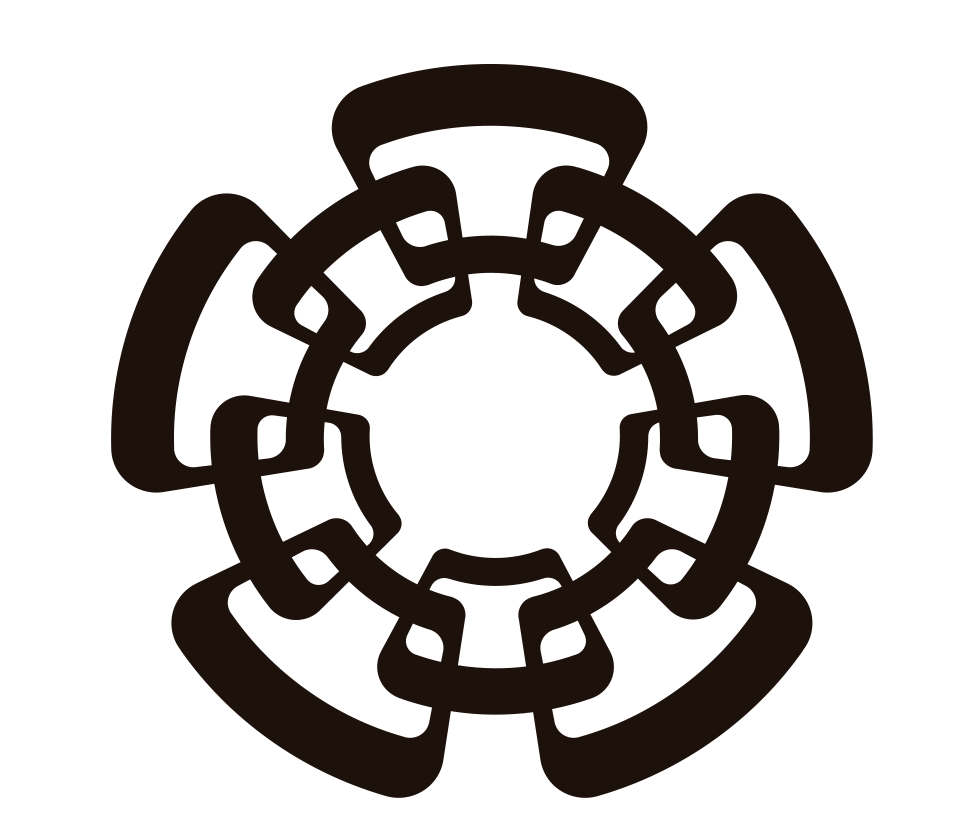
\includegraphics[width=0.23\textwidth]{figures/LogoCinvestav1Negro2.png}

\begin{large}
Centro de Investigación y de Estudios Avanzados del Instituto Politécnico Nacional\\
\end{large}
\vspace*{2.0cm}
\textbf{\Large DEPARTAMENTO DE FÍSICA}\\
\vspace*{1.5cm}
\begin{large}
TRABAJO FIN DE GRADO
\end{large}

\vspace*{0.1in}
\textbf{\LARGE \tfgTitle}

\vspace*{.2in}

{\large Realizado por}\\
\textbf{\Large \tfgAuthors}

\vspace*{1cm}

\textbf{Para la obtención del título de}\\
{\large \tfgDegree}

\vspace*{0.2in}

\textbf{Dirigido por}\\
{\large \tfgSupervisor}\\

\vspace*{0.2in}




\vspace*{.4in}
\textbf{\large Ciudad de México, \tfgMonth \hspace{0.1cm} de \tfgYear}

\end{center}

% Dedicatoria
\ifdefined\tfgDedication
    \newpage
    \thispagestyle{empty}
    
    \vspace*{\fill}
    \begin{center}
    \textit{\tfgDedication}
    \end{center}
    \vspace*{\fill}
\fi

\clearpage\setcounter{page}{1} % Comienza a incluir números de página a partir de aquí
\pagenumbering{roman} % En números romanos

\newpage{\ }
\thispagestyle{empty}
    \newpage{\ }
    \thispagestyle{empty}
    \thispagestyle{empty} % Impide que se incluya número de página en la portada
\begin{center}
    


\vspace*{-1cm}

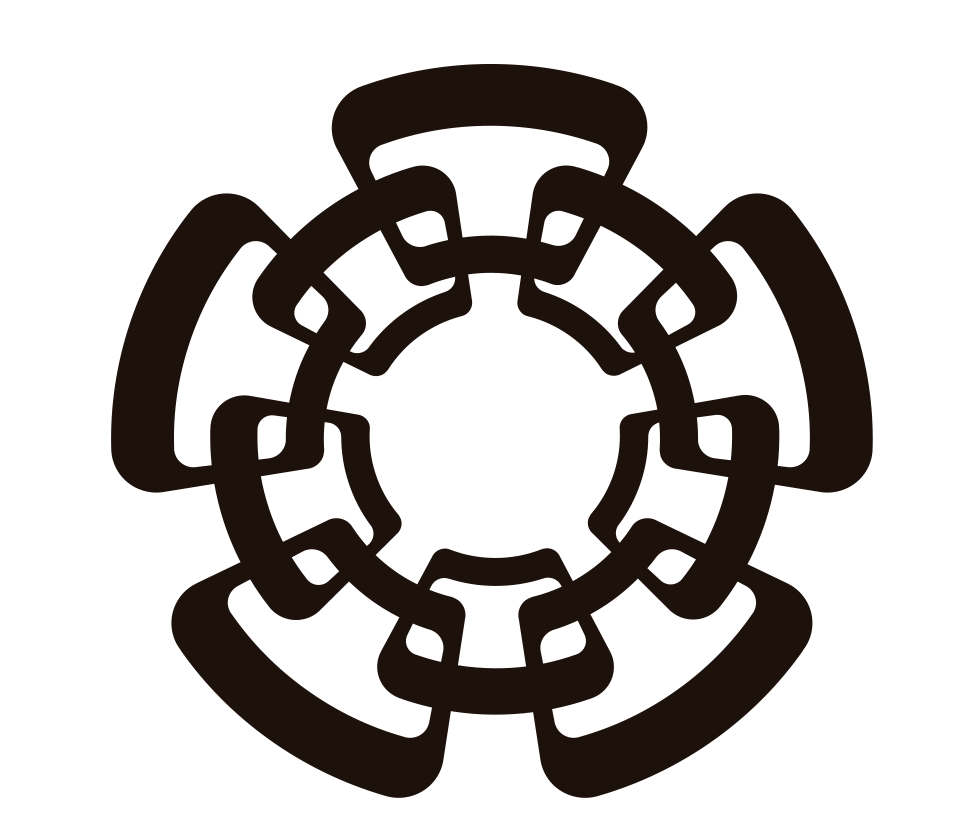
\includegraphics[width=0.23\textwidth]{figures/LogoCinvestav1Negro2.png}
\end{center}
\begin{center}
\begin{large}
Centro de Investigación y de Estudios Avanzados del Instituto Politécnico Nacional\\
\end{large}
\vspace*{2cm}
\textbf{\Large PHYSICS DEPARTMENT}\\
\vspace*{1.5cm}


\textbf{\LARGE Sensitivities to neutrino charge radius at reactor neutrino experiments involving CE$\nu$NS}

\vspace*{.2in}

{\large Presented by}\\
\textbf{\Large \tfgAuthors}

\vspace*{1cm}

\textbf{In order to obtain the}\\
{\large Master of Science degree\\
speciality in Physics}

\vspace*{0.2in}

\textbf{Under the supervision of}\\
{\large PhD Omar Gustavo Miranda Romagnoli}\\

\vspace*{0.2in}




\vspace*{.5in}
\textbf{\large Mexico City, November \hspace{0.1cm} of \tfgYear}

\end{center}

% Dedicatoria
\ifdefined\tfgDedication
    \newpage
    \thispagestyle{empty}
    
    \vspace*{\fill}
    \begin{center}
    \textit{\tfgDedication}
    \end{center}
    \vspace*{\fill}
\fi

\clearpage\setcounter{page}{1} % Comienza a incluir números de página a partir de aquí
\pagenumbering{roman} % En números romanos
}
    \newpage{\ }
    \thispagestyle{empty}
    \chapter*{Agradecimientos}

\textit{agradecimiento aqui.}
    \newpage{\ }
    \thispagestyle{empty}
    \chapter*{Resumen}

El Modelo Estándar (ME) y la teoría electrodébil (EW, por sus siglas en inglés), así como las correcciones radiativas al ángulo de Weinberg ($\sin^2\theta_W$), predicen que los neutrinos, aunque eléctricamente neutros, poseen propiedades electromagnéticas cuantificables. Específicamente, una de estas propiedades es el radio de carga del neutrino (NCR, por sus siglas en inglés). Presentamos cómo diferentes configuraciones experimentales que involucran antineutrinos de reactor interactuando vía Dispersión Elástica Coherente Neutrino-Núcleo (CE$\nu$NS, por sus siglas en inglés) en argón líquido (LAr) pueden obtener resultados diferentes dependiendo de los valores de $\sin^2\theta_W$ y del NCR, cuantificando así la sensibilidad de dichos experimentos a estos parámetros del ME. Los resultados muestran la sensibilidad proyectada de experimentos basados en reactor cerca de la Ciudad de México para determinar el ángulo de Weinberg y el NCR del neutrino electrónico. Encontramos que la precisión proyectada en ambos parámetros escala de forma cercana a $1/\sqrt{N}$ con el tiempo de exposición y mejora en casi un orden de magnitud a lo largo de las masas de detector consideradas, de 10 a 200 kg, mientras que la inclusión de un factor de quenching realista para el argón, en lugar de una respuesta unitaria idealizada, degrada la sensibilidad a ambos parámetros por un factor de dos a tres debido a la pérdida de eventos de retroceso de baja energía por debajo del umbral. Incluso bajo este escenario realista, se proyecta que un detector de 200 kg expuesto durante 200 días restrinja $\sin^2\theta_W$ al nivel de $1$-$2\%$ y el radio de carga del neutrino electrónico a $\langle r_{\nu_e}^2\rangle \sim 2\times10^{-33}\ \text{cm}^2$, una precisión competitiva con las determinaciones de baja energía existentes del ángulo de mezcla débil y un objetivo concreto y comprobable para la estructura electromagnética del neutrino electrónico utilizando una fuente y una tecnología de detección ya disponibles a escala de un laboratorio nacional.

    \newpage{\ }
    \thispagestyle{empty}
    \chapter*{Abstract}
Standard Model (SM) electroweak theory (EW) and radiative corrections to the Weinberg angle ($\sin^2\theta_W$) predict that neutrinos, while electrically neutral, possess quantifiable electromagnetic properties. Specifically, one such property is the neutrino charge radius (NCR). We present how different experimental configurations involving reactor antineutrinos interacting via Coherent Elastic Neutrino-Nucleus Scattering (CE$\nu$NS) in liquid argon (LAr) can yield differing results depending on the values of $\sin^2\theta_W$ and the NCR, thus quantifying the sensitivity of such experiments to these SM parameters. The results show the projected sensitivity of reactor-based experiments near Mexico City to determining the Weinberg angle and the electron-neutrino NCR. We find that the projected precision on both parameters scales close to $1/\sqrt{N}$ with exposure time and improves by nearly an order of magnitude across the detector masses considered, from 10 to 200 kg, while the inclusion of a realistic quenching factor for argon, rather than an idealized unit response, degrades the sensitivity to both parameters by a factor of two to three due to the loss of low-energy recoil events below threshold. Even under this realistic scenario, a 200 kg detector exposed for 200 days is projected to constrain $\sin^2\theta_W$ to the $1$-$2\%$ level and the electron-neutrino charge radius to $\langle r_{\nu_e}^2\rangle \sim 2\times10^{-33}\ \text{cm}^2$, a precision competitive with existing low-energy determinations of the weak mixing angle and a concrete, testable target for the electron-neutrino electromagnetic structure using a source and detector technology already available at a national laboratory scale.

    \newpage{\ }
    \thispagestyle{empty}
    
    % Índice del documento y de figuras
    \begingroup

        \hypersetup{linkcolor=black}
        \tableofcontents
        %\listoffigures
        %\listoftables
        %\lstlistoflistings
    \endgroup
    
    % Cambia el estilo de números de página de romanos a normal
    \clearpage\pagenumbering{arabic}
    

    % Capítulos del trabajo
    \chapter{Introduction}
\label{chap:introduction}

Particle physics is dedicated to unraveling the most fundamental constituents of the universe and the forces that govern their interactions. It explores the known elementary particles, such as quarks, leptons, and bosons, which constitute matter and mediate the fundamental forces, and it organizes them within the Standard Model (SM), the central theoretical framework of the field. The SM has been remarkably successful in describing the behavior of these particles, yet the discovery that neutrinos have mass and undergo flavor-changing oscillation showed that the model, in its original massless-neutrino formulation, is necessarily incomplete. This has made the neutrino sector one of the most active windows through which physics beyond the Standard Model (BSM) may first reveal itself.

Neutrinos were theoretically proposed by Pauli in 1930 to preserve energy and angular momentum conservation in beta decay, and they were experimentally discovered in 1956 by Cowan and Reines, after decades in which the technology required to detect their exceedingly weak interaction with matter simply did not exist. Since then, neutrinos have been studied in ever greater detail, from the discovery of their oscillations to the ongoing effort to pin down their absolute mass scale, their Dirac or Majorana nature, and their possible electromagnetic properties. Among these properties, the neutrino charge radius (NCR) occupies a particular place: unlike a magnetic moment or an electric dipole moment, it is not an independent addition to the SM but a genuine radiative prediction of electroweak theory itself, arising unavoidably at one loop even in the absence of any new physics. This makes the NCR simultaneously a precision test of the SM and a potential probe of BSM scenarios that would shift its predicted value away from the SM benchmark.

This work focuses on Coherent Elastic Neutrino-Nucleus Scattering (CE$\nu$NS), a process whose cross section is precisely predicted by the SM and is directly sensitive to the electroweak couplings that the NCR modifies. This sensitivity, however, comes with the fact that CE$\nu$NS events correspond to extremely low-energy nuclear recoils, which are experimentally challenging to observe and which must be related, through a detector-dependent quenching factor, to the ionization energy that is actually measured. Furthermore, the shift induced by the NCR on the effective weak coupling is, at leading order, degenerate with a shift in the weak mixing angle $\sin^2\theta_W$ itself, so that any realistic sensitivity study must treat these two SM quantities together rather than in isolation. In this thesis we study the projected sensitivity of a reactor-based CE$\nu$NS experiment using a liquid argon (LAr) target to both $\sin^2\theta_W$ and the electron neutrino charge radius $\langle r_{\nu_e}^2\rangle$, using as a concrete benchmark the SBC-ININ-LAr proposal exposed to the antineutrino flux of the TRIGA Mark III reactor. We show how the interplay between detector mass, exposure time, and the realistic treatment of the quenching response determines how well these two parameters can be constrained, and to what extent their mutual degeneracy can be resolved.

The thesis introduces, in Chapter 2, the electroweak theory of the SM, beginning with a brief history of the neutrino and its role as the catalyst for the proposal and eventual discovery of the weak nuclear force, followed by the unification of that force with electromagnetism into the electroweak theory that underlies all subsequent calculations in this work. In Chapter 3, we turn to radiative corrections within this framework, showing how the inclusion of one-loop diagrams to the effective neutrino-fermion interaction predicts the electromagnetic properties of the neutrino, and in particular the neutrino charge radius, and how this prediction modifies the SM parameters, most notably $\sin^2\theta_W$, that are probed experimentally. Chapter 4 introduces CE$\nu$NS itself as the neutral-current interaction through which these SM parameters are experimentally accessed, presenting its cross section and combining it with a model of the reactor antineutrino flux to compute the expected number of events for a broadly-described experimental design, a quantity that later chapters use to test the influence of different SM parameter values. Chapter 5 presents the projected sensitivity of the SBC-ININ-LAr experiment to $\sin^2\theta_W$ and $\langle r_{\nu_e}^2\rangle$, for a range of detector masses, exposure times, and quenching factor treatments, together with the corresponding $\Delta\chi^2$ confidence intervals. Finally, we give our conclusions in Chapter 6.
    \chapter{Electroweak theory in the Standard Model of particles}\label{cap:introduccion}
\section{Introduction}
\begin{figure}
    \centering
    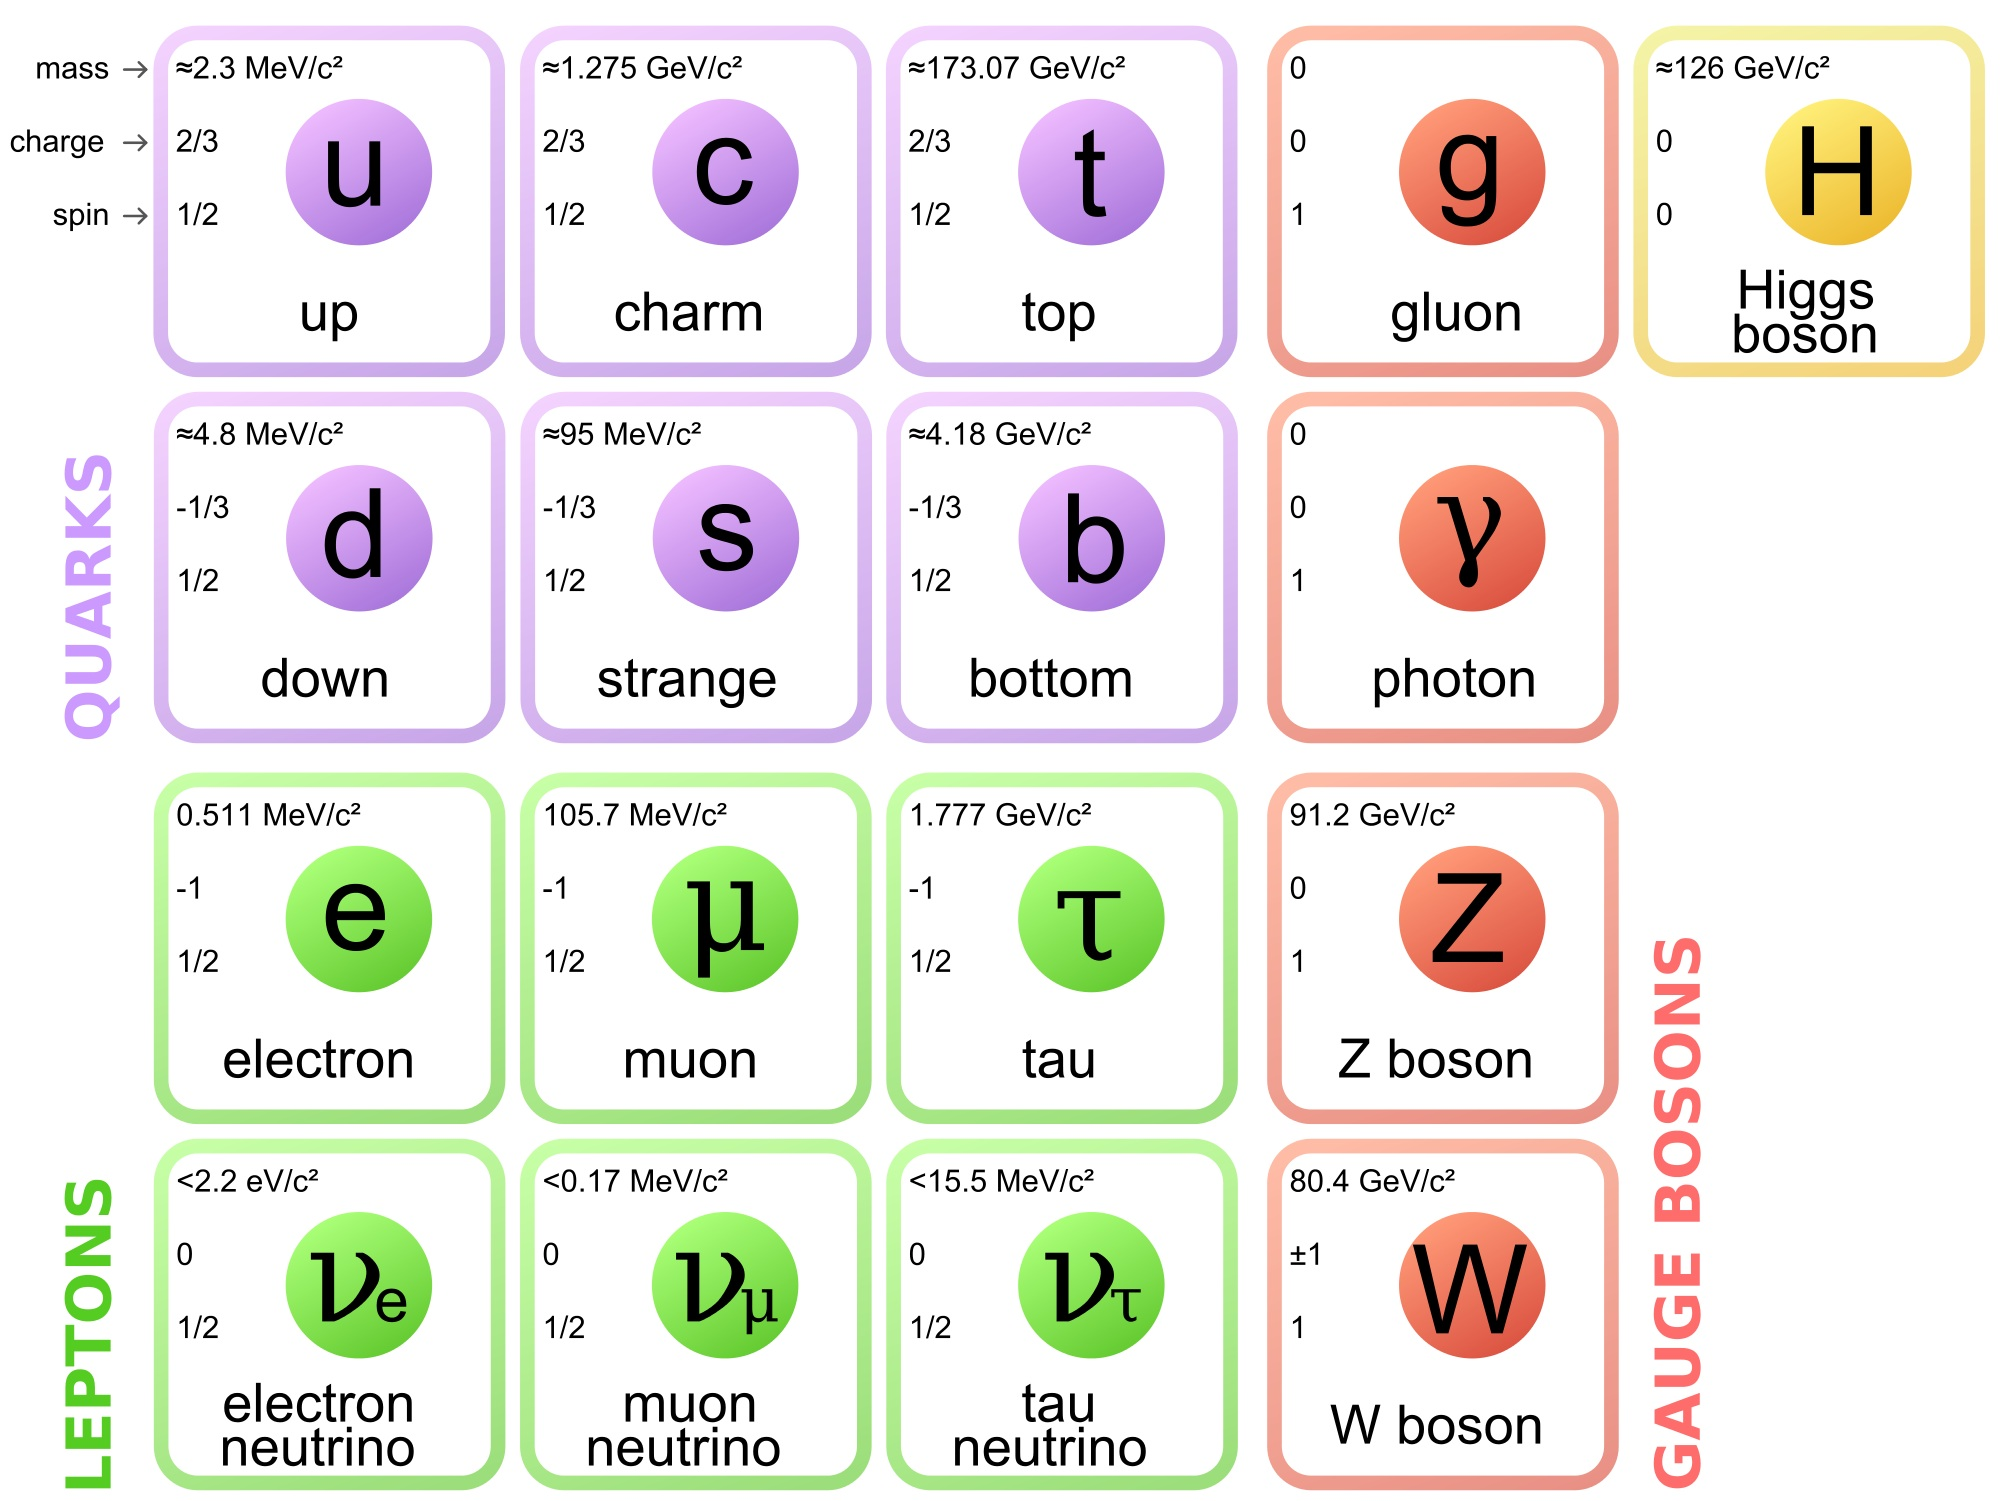
\includegraphics[width=0.8\linewidth]{figures/StandardModel.jpg}
    \caption{Particles in the SM}
    \label{fig:SM}
\end{figure}
The Standard Model of particles (SM) is the most currently utilized theory of interactions of subatomic particles. It describes all 
matter particles and forces between them, excluding gravity, as interactions between 12 fermions (6 quarks and 6 leptons) with their corresponding anti-fermions, 4 spin-1 force-carrying gauge bosons and 1 scalar boson as shown in Fig. \ref{fig:SM}. Within this framework exist 3 distinct forces: strong nuclear force, mediated by the gluon ($g$) boson; electromagnetic (EM) force, mediated by the photon ($\gamma$) boson; and weak nuclear force, mediated by the $W^{\pm}$ and $Z$ bosons. 
This work pertains to the description of the properties of the only family of particles that present no electric or color charge known as neutrinos ($\nu$), wherein the SM exist three known flavors ($\nu_e$, $\nu_\mu$ and $\nu_\tau$) corresponding to the latter half of (electro)weak isospin doublets formed with the known charged leptons ($e^-$, $\mu^-$ and $\tau^-$). This chapter aims to describe neutrinos in the SM, the weak force and its origin as a part of a larger broken symmetry known as "Electroweak Theory" (EW). 
\section{Symmetries and fermion content}
\subsection{Neutrinos}
Neutrinos are charge-less, color-less, spin-$\frac{1}{2}$ particles with negligible masses compared to other fundamental particles first proposed in 1930 by Pauli W.~\cite{pauli1930neutrino}, and later detected by C. L. Cowan et al. in 1956~\cite{doi:10.1126/science.124.3212.103}, to solve known apparent contradictions in conserved quantities of beta decays. Beta decay was known to be as the emission of beta particles (electrons) by the nuclei of unstable atoms, wherein the difference in mass of the original and resulting nuclei of the decay should fix the energy at which the emitted particles are detected. Also of note, due to conservation of angular momentum the sum of the spin ($S_e$) of the electron, the spin of the resulting nucleus ($S_{N^{*}}$) and the angular momentum between them ($L$) should equal the original nucleus' spin ($S_{N}$). Despite this, it was know experimentally that the resulting electrons where emitted in a spectrum of energies less than expected and at $L=0$, making the sum of spins impossible to match.
Pauli's solution to the apparent violation of the conservation of these quantities was to hypothesize the existence of a second neutral spin-$\frac{1}{2}$ with very small mass compared to the electron that allows for both the distribution of energy between both emitted particle, thus letting the electron be emitted at different energies depending on the kinematics, and the conservation of angular momentum. 
\begin{align*}
    N &\rightarrow N^{*} + e^{-}     ~ &\rightarrow&    &N \rightarrow& N^{*} + e^{-} + \nu \\ \hline
    m_N &= m_{N^*} + E_{e^-}         ~ &\rightarrow&   &m_N =& m_{N^*} + E_{e^-} + E_{\nu} \\
    S_{z~N} &= S_{z~N^*} + S_{z~e^-} ~ &\rightarrow&   &S_{z~N} =& S_{z~N^*} + S_{z~e^-} + S_{z~\nu}
\end{align*}
Later refinement of the atomic model found that nuclei where made up of positively charged elements named protons ($p$) and neutrally charged elements known as neutrons\footnote{this was the name first proposed for the particle hypothesized by Pauli, later changed} ($n$), leaving the small hypothesized particle to be named neutrino ($\nu$) later by Enrico Fermi. It is well understood now that the beta decay is a process in which a neutron within an unstable nucleus decays into a proton, an electron and a(n) (anti)neutrino.  
$$n \rightarrow p + e^{-} + \bar{\nu}$$
Subsequent experiments exploiting cross symmetry of the above interaction~\cite{doi:10.1126/science.124.3212.103}, accelerator-produced pion decay~\cite{Danby1962}, and charged-current tau neutrino interactions in nuclear emulsion~\cite{Kodama2001, Kodama2008} confirmed the existence of three distinct active neutrino flavors and the conservation of lepton family number in the interactions that involved these particles. Given that neutrinos don't interact via electromagnetic or strong forces a theory of a different force that mediated these interactions was developed into what is now known as the "weak nuclear force".
\subsection{Weak Nuclear Force}
Developments in quantum mechanics (QM) and special relativity (SR) led up to the first theories that could describe the behavior of some subatomic particles and their interactions through excitations of quantized fields called quantum field theories (QFTs) obtained by promoting classical fields to operator-valued quantities satisfying canonical (anti)commutation relations and deriving their dynamics from a Lorentz-invariant action principle. One of the earliest and most successful QFTs was Quantum Electro Dynamics (QED), describing how spin-1/2 (anti)particles (\stackon[.1pt]{$\psi$}{\brabar}) interacted with an EM 4-potential ($A^\mu$) by minimizing the action given by the lagrangian density: 
\begin{equation}
    \mathcal{L}_{\text{QED}} = \underbrace{\bar{\psi}(i\gamma^\mu\partial_\mu - m)\psi}_{\text{free Dirac field}} - \underbrace{\frac{1}{4}F_{\mu\nu}F^{\mu\nu}}_{\text{free EM field}} - \underbrace{e\bar{\psi}\gamma^\mu\psi A_\mu}_{\text{interaction}}.
    \label{eq:L_QED}
\end{equation}
While the `free' terms in (\ref{eq:L_QED}) describe the propagation of Dirac fermions and photons in free Minkowski space, the `interaction' term describes a vertex that couples the (anti)fermion current with the electromagnetic four-potential, representing the elementary process of a(n) (anti)fermion emitting or absorbing a photon. At zeroth-order $\hbar$ perturbative terms, QED had shown predictive power for processes like Compton ($\gamma + e^- \rightarrow \gamma + e^-$)~\cite{KleinNishina1929} and M\o ller ($e^- + e^- \rightarrow e^- + e^-$)~\cite{Moller1932} scattering by the time Fermi first proposed an interaction inspired by the QED interaction term, where instead of a fermion current emits a photon, two fermion currents meet at a vertex such that a coupling constant (now called Fermi's constant $G_F$) quantified the intensity of the interaction, and thus can be estimated experimentally.
\begin{center}
% https://feynman.srossd.com/#N4Igdg9gJgpgziAXAbVABwnAlgFyxMJZABgBoBGAXVJADcBDAGwFcYkQQBfU9TXfQinIVqdJq3ZceIDNjwEiAJlLFRDFm0QduvOQKWlFa8Zu3TZ-BSmVUa6iVoC8U3ZcHIAzCLsn2AHT9sAFsXGT55dzIAFmMNSR0wvStkYRi7GAAnHBgAD3YoCBxQiwiDD1iHM1dS61I0sTitYvD9WoBWCtNmpPcvevtTAODutyIo7wbKmACAI3oM4AC0bE4AfWAAM04AgHN6IKD6AD0AoOYl7HWtgAIAQVXT5hGa5HH+3y0AgAoAjYz6ADGwAA4qsAGKcRaBACOWWAik4nB+fjmCwuWDWwDA2z8ewOx0e6PWaE4AEpkaiocsMesAmBmDi8YcHn4zkTgDAjsAALSI0kBUnPVokFRqTLZPJaApFBIlYVtOqdfx+P6AkHgyFDWE4eGIinzKkrdbY3b7Q4nVnnPzU4lk-Vo61GqH0xlm+gstmOrDrTk8vlC5IK2yTUzTFEG9GYram-EWz02zacO4ep6cUQwKA7eBEUB-CAhRBkEA4CBIYQgAEAC3mWbLNEY9BmMEYAAUWlYQIwYBsij5GiANqE8wXyyWkMoK9WMrXEOXGFgwKYNpkgvo+5VBwlh3Xi6XEF5OwvTGhK4UFPXG822z12BksDtK72Q8qmfQhxl80gAGw0MeIADsNBVjWmjlgM7BoO+n6IAAHL+e6AZOIFINyYEfOAUEFgAnPBSCIcB06geugzhg6LqYWWRZ-vhU4zqhxHsJy3JcJQnBAA
\begin{tikzpicture}
\begin{feynman}
\vertex (0) at (0, 8);
\vertex (1) at (2, 8);
\vertex (2) at (4, 10);
\vertex (3) at (4, 6);
\vertex (4) at (4, 8);
\vertex (5) at (6, 8) {\(\sim\)};
\vertex (6) at (0, 2);
\node[dot] (7) at (2, 2);
\vertex (8) at (4, 4);
\vertex (9) at (4, 2);
\vertex (10) at (4, 0);
\vertex (11) at (6, 2) {\(\sim\)};
\vertex (12) at (8, 8) {\(e\bar{\psi}_{f}\gamma^\mu\psi_{f} A_\mu\)};
\vertex (13) at (8, 2);
\vertex (18) at (10, 2) {\(\mkern-80mu \frac{G_F}{\sqrt{2}}(\bar{\psi}_{n}\gamma^\mu\psi_{p})(\bar{\psi}_{\nu}\gamma_\mu\psi_{e^{-}})\)};
\vertex (19) at (10, 8);
\diagram*{
	(0) --[fermion,edge label={\(f\)}] (1),
	(1) --[fermion,edge label={\(f\)}] (2),
	(1) --[photon,edge label'={\(\gamma\)}] (3),
	(6) --[fermion,edge label={\(p\)}] (7),
	(8) --[anti fermion,edge label={\(n\)}] (7),
	(9) --[fermion,edge label={\(\bar{\nu}\)}] (7),
	(10) --[anti fermion,edge label={\(e^-\)}] (7)
};
\end{feynman}
\end{tikzpicture}
\end{center}
Subsequent discoveries in particle physics revealed that charged-current weak interactions violate parity symmetry maximally. First theorized by Lee and Yang in 1956~\cite{Lee:1956qn} to resolve the then-known $\tau - \theta$ puzzle, and later verified experimentally by Wu et al. in 1957~\cite{Wu:1957my}, this motivated a modification of the Fermi interaction in the form of a combination of the two bilinear Lorentz-invariant structures that admit such violation~\cite{Sudarshan:1958vf, Feynman:1958ty}.

\begin{align}
\text{V}&:  j_{V}^{\mu} = \bar{\psi}\gamma^\mu\psi &\xrightarrow{\mathcal{P}}& &j'_{V~\mu} &= \bar{\psi}\gamma_\mu\psi& \label{eq:V}\\
\text{A}&:  j_{A}^{\mu} = \bar{\psi}\gamma^\mu\gamma^5\psi &\xrightarrow{\mathcal{P}}& &j'_{A~\mu} &= -\bar{\psi}\gamma_\mu\gamma^5\psi& \label{eq:A}
\end{align}

The expressions (\ref{eq:V}) and (\ref{eq:A}) show how different bilinear structures change under parity ($\mathcal{P}$) and how pure vector (axial) currents are $\mathcal{P}-even$ ($\mathcal{P}-odd$). Given a general current structure, $j^\mu = g_V j_{V}^\mu + g_A j_{A}^\mu$, observables that depend on the inner product of two such currents transform under parity as:
\begin{align}
    |\mathcal{M}|^2 &= (j_{1} \cdot j_{2}) = g_V^2 (j_{1~V} \cdot j_{2~V}) + g_A^2 (j_{1~A} \cdot j_{2~A}) + g_V g_A (j_{1~V} \cdot j_{2~A} + j_{1~A} \cdot j_{2~V})\label{eq:M} \\  \nonumber
    &\xrightarrow{\mathcal{P}} \\
    |\mathcal{M}'|^2 &= (j'_{1} \cdot j'_{2}) = g_V^2 (j'_{1~V} \cdot j'_{2~V}) + g_A^2 (j'_{1~A} \cdot j'_{2~A}) - g_V g_A (j'_{1~V} \cdot j'_{2~A} + j'_{1~A} \cdot j'_{2~V}).\label{eq:Mprime}
\end{align}
The only difference between \ref{eq:M} and \ref{eq:Mprime} lies in the sign of the interference term, such that the degree of $\mathcal{P}$-symmetry violation is given by the coefficient $\frac{g_V g_A}{g_V^2 + g_A^2}$. Normalizing this there are two options for maximally violated $\mathcal{P}$-symmetry given by $\frac{g_V}{g_A} = \pm 1$, also known as $V\pm A$ currents. Given that in the Wu experiment it was determined that (anti)neutrinos are emitted exclusively as left(right)-handed fermions the appropriate structure to use for weak interactions was determined to be $V-A$. Modifying the Fermi lagrangian density for beta decay to include this gives the following expression:
\begin{equation}
    \mathcal{L}_{CC}=\frac{G_{F}}{\sqrt{2}}\left[\bar{\psi}_{\nu_{e}}\gamma^{\mu}(1-\gamma^{5})\psi_{e}\right]\left[\bar{\psi}_{p}\gamma_{\mu}(1-\gamma^{5})\psi_{n}\right]+\text{h.c.} \label{eq:VALag}
\end{equation}
Later refinements of this theory succeeded in demonstrating the universality of the weak interaction across leptonic decays and strangeness-changing meson decays through Cabibbo mixing~\cite{Cabibbo:1963yz}. This not only established that all such processes are mediated by the same underlying force, but also motivated the prediction and subsequent discovery of the charm quark~\cite{Glashow:1970gm}. With these improvements on the theory thus far, the point-like structure of the interaction still led to scattering amplitudes proportional to the center-of-mass energy $\sqrt{s}$, resulting in S-matrix unitarity violation at higher energies. The natural resolution, in analogy with QED, is to conceive of Fermi's interaction as the low-energy limit of a gauge field theory, wherein the maximal parity violation of the charged currents naturally gives rise to three mediating vector bosons corresponding to the generators of an $SU(2)_L$ symmetry, which must be massive due to the short range of the weak interaction. Given this hypothesis, Glashow showed in 1961~\cite{Glashow1961} that the gauge field theory whose low-energy limit reproduces the $V-A$ structure of charged currents requires a $SU(2)_L \times U(1)_Y$ symmetry group, which not only predicted the existence of neutral weak currents, later measured in 1973 at the GARGAMELLE experiment at CERN~\cite{Hasert1973a, Hasert1973b},  but also unified the weak and electromagnetic interactions into a single electroweak theory, later developed independently by Weinberg and Salam~\cite{Weinberg1967, Salam1968}.
\section{Massive and Massless Mediators}

\section{Electroweak mixing $\sin^2 \theta_W$}



    \chapter{Radiative Corrections and Neutrino Charge Radius}\label{cap:NCR}
This chapter is concerned with the main theoretical focus of this work. The SM as described in Chapter \ref{cap:EWinSM}, and in specific EW theory within it, models the interactions between fermions and gauge bosons utilizing of perturbative terms in the from of higher-order loop diagrams. While tree level calculations offered good agreement with experimental data, modern precision in particle experiments have required in recent history have shown the necessity to include higher-order terms to either validate the SM or in occasions point to scenarios Beyond the SM (BSM). This chapter describes how the inclusion of 1-loop diagrams to an effective interaction reveal predictions of electromagnetic properties of the neutrino and how they modify previously established parameters in the SM.

\section{Introduction}
The electromagnetic properties of the neutrino were not only essential to its first postulation and subsequent discovery, but remain an active field of research in modern experimental particle physics. Indeed, both its neutral charge and the possibility of a non-zero magnetic dipole moment are mentioned in the original 1930 letter by Pauli that first introduced the neutrino~\cite{pauli1930neutrino}. The study of such properties was further motivated by the proposal and eventual discovery of neutrino flavor oscillations and their requisite non-zero mass splittings. This chapter describes how radiative corrections to the effective $\nu\nu\gamma$ vertex predict non-trivial electromagnetic form factors for massive\footnote{This chapter concerns primarily Dirac-type neutrinos; analogous calculations for Majorana neutrinos can be found in~\cite{PhysRevD.26.3152, PhysRevD.26.1662, RevModPhys.87.531}} neutrinos within the SM, the focus of this work being the neutrino charge radius (NCR).

\section{Electromagnetic Form Factors}\label{sec:EMFF}
\subsection{Massive Neutrinos}

\begin{figure}\label{fig:vertices}
\centering 
\subfigure[]{\label{subfig:a}\resizebox{0.3\textwidth}{!}{\begin{tikzpicture}
\begin{feynman}
\vertex (0) at (0, 4){\(\mathfrak{f}(p_i)\)};
\vertex (1) at (2, 2);
\vertex (2) at (4, 4){\(\mathfrak{f}(p_f)\)};
\vertex (3) at (2, 0){\(\gamma(q)\)};
\diagram*{
	(0) --[fermion] (1),
	(1) --[fermion] (2),
	(1) --[photon] (3)
};
\end{feynman}
\end{tikzpicture}}}\hfil
\subfigure[]{\label{subfig:b}\resizebox{0.3\textwidth}{!}{\begin{tikzpicture}
\begin{feynman}
\vertex (0) at (0, 4){\(\nu(p_i)\)}; ;
\node[draw, circle, minimum size=1.5em] (1) at (2, 2){\(\Lambda_\mu\)};
\vertex (2) at (4, 4){\(\nu(p_f)\)};
\vertex (3) at (2, 0){\(\gamma(q)\)};
\diagram*{
	(0) -- [fermion] (1) ,
	(1) -- [fermion] (2) ,
	(1) -- [photon] (3) 
};
\end{feynman}
\end{tikzpicture}}}\hfil
\subfigure[]{\label{subfig:c}\resizebox{0.3\textwidth}{!}{\begin{tikzpicture}
\begin{feynman}
\vertex (0) at (0, 4){\(\nu^j(p_j)\)}; ;
\node[draw, circle, minimum size=1.5em] (1) at (2, 2){\(\Lambda_\mu^{kj}\)};
\vertex (2) at (4, 4){\(\nu^k(p_k)\)};
\vertex (3) at (2, 0){\(\gamma(q)\)};
\diagram*{
	(0) -- [fermion] (1) ,
	(1) -- [fermion] (2) ,
	(1) -- [photon] (3) 
};
\end{feynman}
\end{tikzpicture}}}
\caption{my caption}
\end{figure}

Following Ref.~\cite{RevModPhys.87.531}, the interaction between a fermionic field $\mathfrak{f}(x)$ and the electromagnetic field $A^\mu$ in the SM is given by the interaction Hamiltonian
\begin{equation}\label{eq:Hem}
	\mathcal{H}_{\text{EM}}(x) = j^{\mathfrak{f}}_{\mu}(x)A^\mu(x) = q_{\mathfrak{f}}\,\bar{\mathfrak{f}}(x)\gamma_\mu\mathfrak{f}(x)A^\mu(x),
\end{equation}
where $q_\mathfrak{f}$ is the electric charge of a fermion $\mathfrak{f}$. Fig. \ref{subfig:a} shows the corresponding the tree-level Feynman diagram for (\ref{eq:Hem}) where the photon $\gamma$ is the quanta of the EM field $A^\mu$. For the neutrino no such direct interaction term exists due to its neutral charge. Nevertheless, at the quantum level such interactions can arise when including higher order terms in the perturbative expansion of interaction terms in the form of loop diagrams. In the 1-photon approximation the effective interaction Hamiltonian for a massive neutrino $\nu$ is given by
\begin{equation}\label{eq:Heffem}
	\mathcal{H}^{(\nu)}_{\text{EM}}(x) = j^{(\nu)}_{\mu}(x)A^\mu(x) = \bar{\nu}(x)\Lambda_\mu\nu(x)A^\mu(x),
\end{equation}
where $j^{(\nu)}_{\mu}(x)$ is the effective neutrino current and $\Lambda_\mu$ is a $4\times4$ vertex function matrix in spinor space which can contain space-time derivatives such that $j^{(\nu)}_{\mu}(x)$ transforms as a four-vector. The corresponding effective Feynman diagram for (\ref{eq:Heffem}) is shown in Fig. \ref{subfig:b}. We will see that the neutrino electromagnetic form factors and properties such as charge and magnetic dipole will correspond to the Fig. \ref{subfig:b} interaction, but it is worth contrasting the origin of these form factors with the analogous quantities for composite particles such as the proton or the neutron, where electromagnetic form factors encode genuine information about the spatial distribution of fundamental constituents. The neutrino carries no such substructure; its form factors are instead radiative effects generated by quantum loops involving gauge bosons. They are physical and, in principle, measurable, but they constitute effective electromagnetic properties induced by the weak interaction rather than a reflection of any internal composition. In this sense the neutrino electromagnetic form factors occupy a conceptually distinct place within the Standard Model. \\
We are intrested in the neutrino part of the Fig. \ref{subfig:b} interaction amplitude, given by the matrix element
\begin{equation}\label{eq:matrixel}
	\bra{\nu(p_f,h_f)}j^{(\nu)}_{\mu}(x)\ket{\nu(p_i,h_i)},
\end{equation}
where $p_{i(f)}$ and $h_{i(f)}$ denote the momentum and helicity of the initial (final) neutrino respectively. Setting aside the helicity dependence for now and taking into account
\begin{equation}\label{eq:canonicalderivative}
	\partial^\mu j^{(\nu)}_\mu = i \left[ \mathcal{P}^\mu, j^{(\nu)}_\mu\right],
\end{equation}
where $\mathcal{P}^\mu$ is the four-momentum operator which generates translations, the effective neutrino current can be rewritten as
\begin{equation}\label{eq:jPnu}
	j^{(\nu)}_\mu(x) = e^{i\mathcal{P}\cdot x}j^{(\nu)}_\mu(0)e^{-i\mathcal{P}\cdot x}.
\end{equation}
Since $\mathcal{P}^\mu \ket{\nu(p_{i(f)})} = p_{i(f)}^\mu \ket{\nu(p_{i(f)})}$ substituting (\ref{eq:jPnu}) into (\ref{eq:matrixel}) gives
\begin{equation}\label{eq:matrixel2}
	\bra{\nu(p_f)}j^{(\nu)}_{\mu}(x)\ket{\nu(p_i)} = e^{(p_f - p_i)\cdot x}\bra{\nu(p_f)}j^{(\nu)}_{\mu}(0)\ket{\nu(p_i)}.
\end{equation}
It is evident from (\ref{eq:matrixel2}) that the quantity encoding the neutrino--photon interaction is the matrix element $\bra{\nu(p_f)}j^{(\nu)}_{\mu}(0)\ket{\nu(p_i)}$. Since $\ket{\nu(p_i)}$ and $\bra{\nu(p_f)}$ describe incoming and outgoing free Dirac particles whose field admits the Fourier expansion
%
\begin{equation}
\psi(x) = \int \frac{d^3p}{(2\pi)^3 2E}\sum_{h=\pm}
\left[ a^{(h)}(p)\,u^{(h)}(p)\,e^{-ix\cdot p}
   + b^{(h)\dagger}(p)\,v^{(h)}(p)\,e^{ix\cdot p}\right],
\end{equation}
%
the only spinor structures that survive in (\ref{eq:matrixel2}) are those sandwiched between free-particle spinors, so that
%
\begin{equation}\label{eq:matrixelem}
\bra{\nu(p_f)}j^{(\nu)}_{\mu}(0)\ket{\nu(p_i)}
= \bar{u}(p_f)\,\Lambda_\mu(p_f,p_i)\,u(p_i).
\end{equation}
%
Here $\Lambda_\mu$ is a $4\times 4$ matrix in spinor space whose free Lorentz index must transform as a contravariant four-vector. The most general such matrix constructed from $\gamma$-matrices and the available four-momenta $p_{i,f}$, or equivalently from $P_\mu = (p_f+p_i)_\mu$ and $q_\mu = (p_f - p_i)_\mu$, is~\cite{Nowakowski_2005}
%
\begin{equation}\label{eq:sixformfactors}
\Lambda_\mu = \varmathbb{f}_1(q^2)\,q_\mu
      + \varmathbb{f}_2(q^2)\,q_\mu\gamma_5
      + \varmathbb{f}_3(q^2)\,\gamma_\mu
      + \varmathbb{f}_4(q^2)\,\gamma_\mu\gamma_5
      + \varmathbb{f}_5(q^2)\,\sigma_{\mu\nu}q^{\nu}
      + \varmathbb{f}_6(q^2)\,\epsilon_{\mu\nu\rho\lambda}\,q^{\nu}\sigma^{\rho\lambda},
\end{equation}
where $\varmathbb{f}_{k}$ ($k=1,\cdots,6$) are six Lorentz-invariant form factors and $q$ is the four-momentum transferred to the photon. Its worth noting that $q^2$ is the only available independent Lorentz-invariant kinematic quantity since $(p_i + p_f)^2 = 4m_{\nu}^2 - q^2$ and thus the vertex function $\Lambda_\mu(q)$ can be written as only dependent on $q$. Further restrictions on $\Lambda_\mu(q)$ are seen when taking into account that $\mathcal{H}^{(\nu)}_{\text{EM}} = \mathcal{H}^{(\nu)\dagger}_{\text{EM}}$ and $A_\mu = A_\mu^\dagger$ thus
\begin{align}
	\bra{\nu(p_f)}j^{(\nu)}_{\mu}(0)\ket{\nu(p_i)} &= \bra{\nu(p_f)}j^{(\nu)}_{\mu}(0)\ket{\nu(p_i)}^\dagger\\
	\implies \bar{u}(p_f)\,\Lambda_\mu(q)\,u(p_i) &= \left(\bar{u}(p_f)\,\Lambda_\mu(q)\,u(p_i)\right)^\dagger\\\label{eq:HermitianL}
	\implies \Lambda_\mu(q) &= \gamma^0 \Lambda_\mu^\dagger(-q) \gamma^0.
\end{align}
Substituting (\ref{eq:HermitianL}) into (\ref{eq:sixformfactors}) constraints the form factor functions such that
\begin{equation}\label{eq:arereal}
	\varmathbb{f}_2,\,\varmathbb{f}_3,\,\varmathbb{f}_4~\text{are real}
\end{equation}
and 
\begin{equation}\label{eq:areimag}
	\varmathbb{f}_1,\,\varmathbb{f}_5,\,\varmathbb{f}_6~\text{are imaginary}.
\end{equation}
Furthermore, imposing current conservation $\partial^{\mu}j^{(\nu)}_\mu=0$ required by the EM $U(1)$ gauge invariance on $A^\mu \rightarrow A^\mu + \partial^\mu \varphi(x)$ for any $\varphi(x)$ which leaves (\ref{eq:Amunu}) invariant in combination with (\ref{eq:canonicalderivative}) leads to
\begin{align}
	\bra{\nu(p_f)}\left[ \mathcal{P}^\mu, j^{(\nu)}_\mu(0)\right]\ket{\nu(p_i)} &= 0\\\label{eq:equalzero}
	\implies q^\mu \bar{u}(p_f) \Lambda_\mu (q) u(p_i) &= 0.
\end{align}
Utilizing on-shell conditions for the neutrino spinors $\slashed{p}_{i(f)}u(p_{i(f)}) = m\,u(p_{i(f)})$, the antisymmetry of $\sigma_{\mu\nu}$ and $\epsilon_{\mu\nu\rho\gamma}$ and the anticommutation relation of $\gamma_\mu$ with $\gamma_5$
\vspace{-.25cm}
\begin{align} 
	\nonumber q^\mu \bar{u}(p_f) \Lambda_\mu (q) u(p_i)&= \bar{u}(p_f) [ \varmathbb{f}_1(q^2)\, q^\mu q_\mu
      + \varmathbb{f}_2(q^2)\,q^\mu q_\mu\gamma_5
      + \varmathbb{f}_3(q^2)\,\overbrace{q^\mu \gamma_\mu}^{\slashed{q} = \slashed{p}_i - \slashed{p}_f} \\ \nonumber
      &+ \varmathbb{f}_4(q^2)\,\underbrace{q^\mu \gamma_\mu}_{\slashed{q} = \slashed{p}_i - \slashed{p}_f} \gamma_5
      + \varmathbb{f}_5(q^2)\,\cancelto{0}{q^\mu\sigma_{\mu\nu}q^{\nu}}
      + \varmathbb{f}_6(q^2)\,\cancelto{0}{q^\mu\epsilon_{\mu\nu\rho\lambda}q^{\nu}}\sigma^{\rho\lambda}] u(p_i)
			\\\nonumber
			&=\bar{u}(p_f) [ \varmathbb{f}_1(q^2)\,q^2
      + \varmathbb{f}_2(q^2)\,q^2\gamma_5
      \\ \nonumber
      &+ \varmathbb{f}_3(q^2)\,(\slashed{p}_i - \slashed{p}_f)
			+ \varmathbb{f}_4(q^2)\,(\slashed{p}_i - \slashed{p}_f)\gamma_5] u(p_i)
			\\\nonumber
			\\\nonumber
			&=\bar{u}(p_f) [ \varmathbb{f}_1(q^2)\,q^2
      + \varmathbb{f}_2(q^2)\,q^2\gamma_5
      \\ \nonumber
      &+ \varmathbb{f}_3(q^2)\,\cancelto{0}{(m - m)}
			+ \varmathbb{f}_4(q^2)\,(m + m)\gamma_5] u(p_i)
			\\\nonumber
			\\\label{eq:operators}
			&=\bar{u}(p_f) [ \varmathbb{f}_1(q^2)\,q^2
							+ \varmathbb{f}_2(q^2)\,q^2\gamma_5
							+ 2m\,\varmathbb{f}_4(q^2)\gamma_5] u(p_i).
\end{align}
Substituting (\ref{eq:operators}) into (\ref{eq:equalzero})
\begin{equation}
	\implies  \varmathbb{f}_1(q^2)\,q^2 + \varmathbb{f}_2(q^2)\,q^2\gamma_5 + 2m\,\varmathbb{f}_4(q^2)\gamma_5 = 0.
\end{equation}
Taking into account that $\mathbb{I}$ and $\gamma_5$ are linearly independent leaves $\varmathbb{f}_1(q^2) = 0$ and $\varmathbb{f}_4(q^2) = -\frac{q^2}{2m} \varmathbb{f}_2(q^2)$. Substituting back into (\ref{eq:sixformfactors}) leaves
\begin{equation}\label{eq:EMformfactors}
	\Lambda_\mu(q) = \varmathbb{f}_Q(q^2)\gamma_\mu -\varmathbb{f}_{M}(q^2)i\sigma_{\mu\nu}q^\nu + \varmathbb{f}_E(q^2)\sigma_{\mu\nu}q^\nu\gamma_5 + \varmathbb{f}_A(q^2)(q^2\gamma_\mu-q_\mu\slashed{q})\gamma_5,
\end{equation}
where $\varmathbb{f}_Q = \varmathbb{f}_3$, $\varmathbb{f}_M = i\varmathbb{f}_5$, $\varmathbb{f}_E = -2i\varmathbb{f}_6$ and $\varmathbb{f}_A=-\varmathbb{f}_2/2m$ are the real charge, dipole magnetic and electric, and anapole neutrino form factors. For the coupling with the real photon at $q^2=0$
\begin{equation}
	\varmathbb{f}_Q(0) = \varmathbb{q},~~~~~~~~~~\varmathbb{f}_M(0) = \mu,~~~~~~~~~~\varmathbb{f}_E(0) = \epsilon,~~~~~~~~~~\varmathbb{f}_A(0) = \varmathbb{a},
\end{equation}
where $\varmathbb{q}$ is the electric charge, $\mu$ the magnetic dipole, $\epsilon$ the electric dipole and $\varmathbb{a}$ the anapole moment of the neutrino. 

\subsection{Massive Neutrino Mixing}
It is worth noting that we have only considered the effective interaction of a single mass eigenstate neutrino with the photon, whereas a full treatment of the known mass mixing among neutrinos requires promoting the aforementioned vertex function and form factors into $N\times N$ matrices, where $\{\ket{\nu_k}\}$, $k=1,2,\cdots,N$, describe $N$ neutrino mass eigenstates of definite mass satisfying $(i\slashed{\partial}-m_k)\nu_k=0$. A generalized version of (\ref{eq:Heffem}), described by the effective Feynman diagram in Fig.~\ref{subfig:c}, is given by
\begin{equation}\label{eq:Heffemkj}
\mathcal{H}^{(\nu)}_{\text{EM}}(x) = j^{(\nu)}_{\mu}(x)A^\mu(x) = \sum_{k,j=1}^{N}\overline{\nu_k}(x)\Lambda^{kj}_\mu\nu_j(x)A^\mu(x),
\end{equation}
where, for an initial state $\ket{\nu_i(p_i)}$ and a final state $\ket{\nu_f(p_f)}$ describing free mass-eigenstate neutrinos, the generalized form of the matrix element in (\ref{eq:matrixelem}) reads
\begin{equation}\label{eq:matrixelemfi}
\bra{\nu_f(p_f)}j^{(\nu)}_{\mu}(0)\ket{\nu_i(p_i)} = \overline{\nu_f}(p_f)\,\Lambda^{fi}_\mu(p_f,p_i)\,\nu_i(p_i).
\end{equation}
As was the case for $\Lambda_\mu(p_f,p_i)$, the matrix $\Lambda^{fi}_\mu(p_f,p_i)$ depends only on $q$ for the same underlying reason, and in its most general form is a linear combination of the same covariant elements, namely
\begin{equation}\label{eq:sixformfactorsfi}
\begin{split}
\Lambda^{fi}_\mu &= \varmathbb{f}^{fi}_1(q^2)\,q_\mu
+ \varmathbb{f}^{fi}_2(q^2)\,q_\mu\gamma_5
+ \varmathbb{f}^{fi}_3(q^2)\,\gamma_\mu\\
&+ \varmathbb{f}^{fi}_4(q^2)\,\gamma_\mu\gamma_5
+ \varmathbb{f}^{fi}_5(q^2)\,\sigma_{\mu\nu}q^{\nu}
+ \varmathbb{f}^{fi}_6(q^2)\,\epsilon_{\mu\nu\rho\lambda}\,q^{\nu}\sigma^{\rho\lambda},
\end{split}
\end{equation}
with conditions (\ref{eq:arereal}) and (\ref{eq:areimag}) holding for the corresponding $\varmathbb{f}^{fi}_m$, $m=1,\cdots,6$. Imposing current conservation, the on-shell conditions for the neutrino spinors $\overline{\nu_f}\slashed{q}\nu_i = \overline{\nu_f}(m_f-m_i)\nu_i$ and the algebraic properties of the covariant forms appearing in (\ref{eq:sixformfactorsfi}) yields the constraints
\begin{numcases}{\left.\right.}
\varmathbb{f}^{fi}_1(q^2) + (m_f-m_i)\varmathbb{f}^{fi}_3(q^2) = 0, & \label{eq:m-m}
\\
\varmathbb{f}^{fi}_2(q^2) + (m_f+m_i)\varmathbb{f}^{fi}_4(q^2) = 0. & \label{eq:m+m}
\end{numcases}
so that the vertex function (\ref{eq:EMformfactors}) is correspondingly promoted to
\begin{equation}\label{eq:EMformfactorsmatrix}
\Lambda^{fi}_\mu(q) = (\gamma_\mu - q_\mu\slashed{q}/q^2)(\varmathbb{f}^{fi}_Q(q^2) + \varmathbb{f}^{fi}_A(q^2)q^2\gamma_5) - i\sigma_{\mu\nu}q^{\nu}(\varmathbb{f}^{fi}_M(q^2)+i\varmathbb{f}^{fi}_E(q^2)\gamma_5),
\end{equation}
where $\varmathbb{f}^{fi}_Q = \varmathbb{f}^{fi}_3$, $\varmathbb{f}^{fi}_M = i\varmathbb{f}^{fi}_5$, $\varmathbb{f}^{fi}_E = -2i\varmathbb{f}^{fi}_6$, and $\varmathbb{f}^{fi}_A = -\varmathbb{f}^{fi}_2/(m_f+m_i)$, subject to the Hermiticity condition
\begin{equation}
\varmathbb{f}^{fi}_{\Omega} = (\varmathbb{f}^{if}_{\Omega})^* \qquad (\Omega = Q,\,E,\,M,\,A).
\end{equation}

Coupling with the real photon at $q^2 = 0$

\begin{equation}
	\varmathbb{f}^{fi}_Q(0) = \varmathbb{q}^{fi},~~~~~~~~~~\varmathbb{f}^{fi}_M(0) = \mu^{fi},~~~~~~~~~~\varmathbb{f}^{fi}_E(0) = \epsilon^{fi},~~~~~~~~~~\varmathbb{f}^{fi}_A(0) = \varmathbb{a}^{fi},
\end{equation}

where $\varmathbb{q}^{fi}$ is the electric charge, $\mu^{fi}$ the magnetic dipole, $\epsilon^{fi}$ the electric dipole and $\varmathbb{a}^{fi}$ the anapole transition moment of an initial $\ket{\nu_i}$ and final $\ket{\nu_f}$ neutrino mass eigenstate. 

It is worth noting that the diagonal entries $f=i$ of $\varmathbb{f}^{fi}_\Omega$ and $\Lambda^{fi}_\mu(q)$ reduce to their single mass-eigenstate counterparts found previously, whereas the off-diagonal entries $f\neq i$ describe transition electromagnetic properties between distinct mass eigenstates, a feature entirely absent in the single-flavor treatment and one of the principal new phenomena introduced by neutrino mixing.

\subsection{Flavor Base}
It is important to recognize, however, that the mass eigenstates $\ket{\nu_i}$ are not the states that are produced or detected in weak interaction processes; rather, it is the flavor eigenstates $\ket{\nu_\alpha}$, $\alpha = e,\mu,\tau$, that couple directly to the charged leptons through the $W^\pm$ boson, the two bases being related by the leptonic mixing matrix $U$ through $\ket{\nu_\alpha} = \sum_i U^*_{\alpha i}\ket{\nu_i}$, better known as the PMNS matrix \cite{10.1143/PTP.28.870, JWFValle_2006}. Consequently, the electromagnetic vertex function in the flavor basis, $\widetilde\Lambda^{\alpha\beta}_\mu$, is obtained from $\Lambda^{ij}_\mu$ by the corresponding unitary rotation
\begin{equation}\label{eq:flavorrotation}
\widetilde\Lambda^{\alpha\beta}_\mu(q) = \sum_{i,j=1}^{3} U_{\alpha i}\,\Lambda^{ij}_\mu(q)\,U^*_{\beta j},
\end{equation}
with the inverse relation $\Lambda^{ij}_\mu = \sum_{\alpha,\beta} U^*_{\alpha i}\,\widetilde\Lambda^{\alpha\beta}_\mu\,U_{\beta j}$ following immediately from the unitarity of $U$. While the algebraic structure of (\ref{eq:EMformfactorsmatrix}) is preserved under this rotation and thus the EM form factors can be definned in the flavor basis such that
\begin{equation}\label{eq:flavorrotation}
\widetilde f^{\alpha\beta}_\Omega(q^2) = \sum_{i,j=1}^{3} U_{\alpha i}\,\varmathbb{f}^{ij}_\Omega(q^2)\,U^*_{\beta j},
\end{equation}
the flavor basis offers no particular simplification on its own; rather, its utility becomes apparent once the calculation of the SM electroweak loop diagrams generating $\Lambda_\mu$ is undertaken, since it is precisely in this basis that the relevant interaction vertices are diagonal.

\subsection{Weyl Neutrinos}
A further simplification arises upon considering the strictly massless limit\footnote{We will show in later sections that this is consistent with the SM and a good approximation at the energy thresholds considered in this work.}, in which the neutrino mass eigenstates reduce to two-component Weyl fermions and helicity coincides exactly with chirality. In this limit, the physical neutrino exists only as the left-handed projection $\nu_{\alpha,\beta(i,j)L}$, while the corresponding antineutrino is purely right-handed, and no Lorentz transformation can connect the two. Since the bilinears $\sigma_{\mu\nu}q^\nu$ and $\sigma_{\mu\nu}q^\nu\gamma_5$ appearing in (\ref{eq:EMformfactorsmatrix}) are odd under chirality and therefore connect left- to right-handed spinors, their matrix elements between same-chirality Weyl states vanish identically, namely $\overline{\nu_{\alpha(i)L}}\,\sigma_{\mu\nu}q^\nu\,\nu_{\beta(j)L} = \overline{\nu_{\alpha(i)L}}\,\sigma_{\mu\nu}q^\nu\gamma_5\,\nu_{\beta(j)L} = 0$, so that $\widetilde f^{\alpha\beta}_M$ ($\varmathbb{f}^{ij}_M$) and $\widetilde f^{\alpha\beta}_E$ ($\varmathbb{f}^{ij}_E$) are forced to vanish in the massless limit. The vertex function correspondingly collapses to
\begin{equation}\label{eq:Lambdamassless}
\widetilde\Lambda^{\alpha\beta}_\mu(q)\Big|_{m_\nu = 0} = (\gamma_\mu - q_\mu\slashed{q}/q^2)\left(\widetilde f^{\alpha\beta}_Q(q^2) - \widetilde f^{\alpha\beta}_A(q^2)q^2\gamma_5\right),
\end{equation}
leaving the charge and anapole form factors as the only surviving electromagnetic structures available to a Weyl neutrino, consistent with the well-known statement that the magnetic and electric dipole moments of a Dirac neutrino are proportional to its mass and hence vanish identically in this limit. Moreover, since the one-loop SM diagrams contributing to the vertex function in the massless limit involve only same-flavor charged lepton propagators running in the loop, the vertex function is diagonal in the flavor basis: $\widetilde\Lambda^{\alpha\beta}_\mu = 0$ and $\widetilde{f}^{\alpha\beta}_{Q,A} = 0$ for $\alpha \neq \beta$ and each of the diagonal entries correspond to electromagnetic properties specific to each neutrino flavor.
\section{Neutrino Charge Radius}
Even if the neutrino is of neutral net charge, its charge form factor $f_Q({q^2})$ can still hold information as to its interaction with other charged particles. In the "Briet frame", defined by the time coordinate of four-momentum transfer such that $q_0 = 0$, $f_Q({q^2})$ only depends on $|\vec{q}| = \sqrt{-q^2}$ and can be interpreted as the Fourier transform of a spherically symmetric charge distribution $\rho(r)$ where $r=|\vec{r}|$.
\begin{equation}
	f_Q(q^2) = \int \rho(r) e^{-i\vec{q} \cdot \vec{r}} d^3 \vec{r} = \int \rho(r) \frac{\sin(|\vec{q}|r)}{|\vec{q}|r}d^3 \vec{r}.
\end{equation}
Deriving with respect to $q^2 = -|\vec{q}|^2$,
\begin{equation}
\dfrac{d f_Q}{dq^2}	= \int \rho(r) \dfrac{\sin(|\vec{q}|r) - |\vec{q}|\cos(|\vec{q}|r)}{2q^3r} d^3\vec{r},
\end{equation}
and thus taking
\begin{equation}
	\lim_{q^2 \rightarrow 0} \dfrac{d f_Q}{dq^2} = \int \rho(r) \frac{r^2}{6} d^3\vec{r} = \frac{\langle r^2 \rangle}{6}.
\end{equation}
Therefore, the average of the squared radius of the neutrino charge distribution is given by
\begin{equation}\label{eq:NRCfinal}
	\langle r^2 \rangle = 6 \left. \dfrac{d f_Q}{dq^2} \right|_{q^2 = 0}.
\end{equation}
Expanding $f_Q(q^2)$ around $q^2 = 0$ in a Taylor series yields
\begin{align}\nonumber
	\left. f_Q(q^2) \right|_{q \approx 0} &\approx \cancelto{0}{f_Q(0)} + \left. \dfrac{d f_Q}{dq^2} \right|_{q^2 = 0}q^2\\ \label{eq:approx}
										 &\approx \frac{\langle r^2 \rangle}{6}q^2,
\end{align}
and substituting (\ref{eq:approx}) into a matrix element of a conserved current with a vertex function of the from in (\ref{eq:Lambdamassless}) at the same limit gives
\begin{align}\nonumber
	\overline{\nu_L}(p_f)\Lambda^{\text{SM}}_\mu(q)\nu_L(p_i)\Big|_{q^2\approx0} & = \overline{\nu_L}(p_f)(\gamma_\mu - \cancelto{0}{q_\mu \slashed{q}/q^2})(f_Q(q^2) + f_A(q^2)q^2\gamma_5)\nu_L(p_i),\\ \label{eq:approxformfac}
												 & \approx \overline{\nu_L}(p_f)(\gamma_\mu)(\frac{\langle r^2 \rangle}{6} - \varmathbb{a})q^2\nu_L(p_i),
\end{align}
utilizing $\gamma_5 \nu_L = - \nu_L$, $\overline{\nu_L}(p_f)\slashed{q}\nu_L(p_i)=0$, and $f_A(0) = \varmathbb{a}$. Because of the from of $\Lambda^{\text{SM}}_\mu$ implied in (\ref{eq:approxformfac}) it's actually a matter of convention between authors what gets defined as the NCR since defining the total neutrino from factor $F_\nu(q^2)$ such that
\begin{equation}
	\Lambda^{\text{SM}}_\mu(q) = \gamma_\mu F_{\nu}(q^2),
\end{equation}
where $F_{\nu}(q^2) = f_{Q}(q^2) + q^2f_A(q^2)$ acts as such that a SM $\nu\nu\gamma$ effective coupling cannot distinguish between an anapole and a charge from factor contribution at the $q\to0$ limit and thus $F_{\nu}(q^2)\Big|_{q^2\to 0}=f_{Q}(q^2)\Big|_{q^2\to 0}~~\implies~~\varmathbb{a} = -\langle r^2 \rangle /6$ for ultra-relativistic left-hand neutrinos. This results in a redefining of an average square charge radius not in terms of $f_Q$, but rather $F_{\nu}$ as a whole which we will denote $\langle r^2 \rangle^\text{SM}$
\begin{equation}\label{eq:factoroftwo}
	\Lambda^{\text{SM}}_\mu(q) = \gamma_\mu F_{\nu}(q^2) \simeq \gamma_\mu\,q^2\frac{\langle r^2 \rangle^\text{SM}}{6} \simeq \gamma_\mu\,q^2\frac{\langle r^2 \rangle}{3}.
\end{equation}
Different authors report either $\langle r^2 \rangle$ or $\langle r^2 \rangle^\text{SM}$ and thus the literature contains differences of factors of 2 for the NCR as seen from (\ref{eq:factoroftwo}). The usual convention for contemporary neutrino phenomenology, and the one that will be used in this work, is to define 
\begin{equation}\label{eq:trueNCR}
	\langle r^2 \rangle^\text{SM} = +6\frac{dF_\nu(q^2)}{dq^2}\Big|_{q=0},
\end{equation}
and report $\langle r^2 \rangle^\text{SM}$ as the NCR. 
\section{Corrections to the $\nu \nu \gamma$ vertex}
The SM prediction for $\langle r^2 \rangle_{\alpha\alpha} = \langle r^2_{\nu_\alpha} \rangle$ as defined by
\begin{equation} 
	\langle r^2 _{\nu_\alpha}\rangle = +6\frac{d\widetilde f^{\alpha\alpha}}{dq^2}\Big|_{q^2=0}
\end{equation} 
arises at one loop from radiative corrections to the $\nu\nu\gamma$ vertex. Within the pinch technique (PT) framework of~\cite{Bernabeu_2000}, one constructs a gauge-invariant, process-independent effective vertex $\hat{\Gamma}^\mu_{\gamma\nu\bar{\nu}}$ by systematically extracting all longitudinal momenta from the conventional vertex, box, and self-energy diagrams and reassigning the resulting propagator-like pieces via the elementary Ward identities of the theory. The diagrams that contribute to $\hat{\Gamma}^\mu_{\gamma\nu\bar{\nu}}$ after this rearrangement are those in which a virtual $W$ boson carries the photon coupling while the associated charged lepton $\ell_\alpha$ runs in the loop; the remaining diagrams either cancel in the PT procedure or are absorbed into the effective self-energies $\hat{\Pi}^{\mu\nu}_{gZ}$ and $\hat{\Pi}^{\mu\nu}_{ZZ}$, which are instead interpreted as process-independent corrections to the effective weak mixing angle~\cite{Bernabeu_2000}. Crucially, the $W$ vertex is diagonal in flavor, it couples $\nu_\alpha$ exclusively to $\ell_\alpha$, so the loop integral depends only on $m_{\ell_\alpha}$ and $M_W$, and the resulting charge form factor $\widetilde{f}^\alpha_Q(q^2)$ is diagonal in the flavor basis. The Dirac form factor extracted from $\hat{\Gamma}^\mu_{\gamma\nu\bar{\nu}}$ then yields, in the limit $q^2\to 0$\footnote{utilizing the definition in (\ref{eq:trueNCR})}~\cite{Bernabeu_2000},

\begin{equation}
\langle r^2_{\nu_\alpha} \rangle = \frac{\langle r^2_{\nu_\alpha} \rangle^\text{SM}}{2}
= -\frac{G_F}{4\sqrt{2}\,\pi^2}
\left[3 - 2\ln\frac{m_{\ell_\alpha}^2}{M_W^2}\right].
\label{eq:NCR_SM}
\end{equation}

\noindent which is finite, gauge-independent, and depends only on the flavor index $\alpha$ through the charged lepton mass $m_{\alpha}$. 

Numerically, the values of NCR prediction for each known neutrino flavour in the SM are\begin{align}
	\langle r^2_{\nu_e} \rangle^\text{SM} &= -0.83 \times 10^{-32}\,\text{cm}^2,\\
	\langle r^2_{\nu_\mu} \rangle ^\text{SM}&= -0.48 \times 10^{-32}\,\text{cm}^2,\\
	\langle r^2_{\nu_\tau} \rangle^\text{SM} &= -0.30 \times 10^{-32}\,\text{cm}^2.
\end{align}

\section{NCR as a radiative correction of Electroweak Mixing}\label{sec:NCRassin}
With a SM prediction for the effective $\nu\nu\gamma$ vertex now in hand, it is possible to include its contribution in the calculation of a neutral current interaction amplitude between a SM left-handed neutrino and a generic fermion $\mathfrak{f}$ of non-zero electric charge, in the limit $q^2 \ll M_Z^2$. Utilizing the vertices in (\ref{eq:QEDintver}), (\ref{eq:gvga}), where for a left-handed neutrino $g^\nu_V = g^\nu_A = 1/2$, and (\ref{eq:factoroftwo}), now written with the explicit dependence on the electromagnetic coupling constant $e$ that was omitted in Sec.~\ref{sec:EMFF}, as well as the propagators (\ref{eq:photonprop}) with $\xi = 1$ and (\ref{eq:lowlimitprocaprop}),

\begin{align}
\left.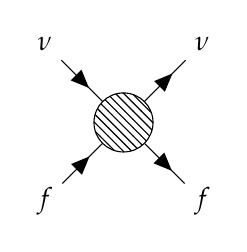
\begin{tikzpicture}[baseline=(3).base]
\begin{feynman}
    \vertex (1) at (0, 0){$\mathfrak{f}$};
	\vertex (2) at (0, 2){$\nu$};
    \node[blob] (3) at (1, 1);
    \vertex (4) at (2, 0){$\mathfrak{f}$};
    \vertex (5) at (2, 2){$\nu$};
    \diagram*{
        (1) --[fermion] (3),
        (2) --[fermion] (3),
        (3) --[fermion] (4),
        (3) --[fermion] (5)
    };
\end{feynman}
\end{tikzpicture}\right.
&\simeq\left.
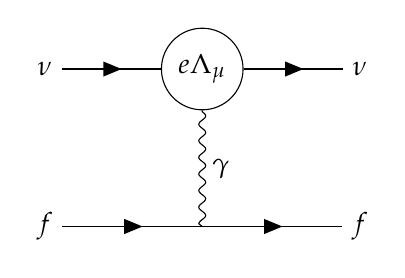
\begin{tikzpicture}[baseline=(7).base]
\begin{feynman}
    \vertex (1) at (0, 0){$\mathfrak{f}$};
	\vertex (2) at (0, 2){$\nu$};
    \node[draw, circle] (3) at (2, 2){$e\Lambda_\mu$};
	\vertex (4) at (2, 0);
    \vertex (5) at (4, 0){$\mathfrak{f}$};
    \vertex (6) at (4, 2){$\nu$};
	\vertex (7) at (1, 1);
    \diagram*{
        (1) --[fermion] (4),
        (2) --[fermion] (3),
		(3) --[boson, edge label=$\gamma$]   (4),
        (4) --[fermion] (5),
        (3) --[fermion] (6)
    };
\end{feynman}
\end{tikzpicture}\right|_{q^2 \ll M_Z^2} + 
\left.
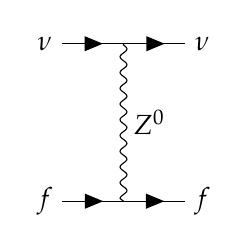
\begin{tikzpicture}[baseline=(7).base]
\begin{feynman}
    \vertex (1) at (0, 0){$\mathfrak{f}$};
	\vertex (2) at (0, 2){$\nu$};
    \vertex (3) at (1, 2);
	\vertex (4) at (1, 0);
    \vertex (5) at (2, 0){$\mathfrak{f}$};
    \vertex (6) at (2, 2){$\nu$};
	\vertex (7) at (1, 1);
    \diagram*{
        (1) --[fermion] (4),
        (2) --[fermion] (3),
		(3) --[boson, edge label=$Z^0$]   (4),
        (4) --[fermion] (5),
        (3) --[fermion] (6)
    };
\end{feynman}
\end{tikzpicture}\right|_{q^2 \ll M_Z^2}\\\nonumber
\implies -i\mathcal{M}&\simeq\left[-ie\overline{\nu_L}\gamma_\mu\,q^2\,\frac{\langle r^2_\nu\rangle^\text{SM}}{6}\nu_L\right]\frac{-i\eta^{\mu\nu}}{q^2}\left[\overline{\mathfrak{f}}-ieQ_{\mathfrak{f}}\gamma_{\nu}\mathfrak{f}\right]\\ \label{eq:firstamplitude}&+\left[\frac{-ig}{2\cos \theta_W}\overline{\nu_L}\gamma_\mu(\frac{1}{2}-\frac{1}{2}\gamma_5)\nu_L\right]\frac{+i\eta^{\mu\nu}}{M_Z^2}\left[\frac{-ig}{2\cos \theta_W}\overline{\mathfrak{f}}\gamma_\mu(g^{\mathfrak{f}}_V-g^{\mathfrak{f}}_V\gamma_5)\mathfrak{f}\right].
\end{align}

\noindent One can observe from (\ref{eq:firstamplitude}) that the $q^2$ dependence of $\Lambda_\mu$ cancels exactly against the photon propagator, so that even in the low-energy limit the electromagnetic form factors survive. Taking into account that $\nu_L = \frac{1}{2}(1-\gamma_5)\nu_L$, together with (\ref{eq:coupling}) and (\ref{eq:MWMZrelation}), further simplifications yield
%
\begin{align}\nonumber
\mathcal{M} &= \underbrace{\left[e\overline{\nu_L}\gamma_\mu\nu_L\right]}_{=\overline{\nu_L}e\gamma_\mu\frac{1}{2}(1-\gamma_5)\nu_L}\left[\overline{\mathfrak{f}}\frac{e\langle r^2_\nu\rangle^\text{SM}Q_\mathfrak{f}}{6}\gamma^\mu \mathfrak{f}\right] - \underbrace{\frac{g^2}{8\cos^2 \theta_W M_Z^2}}_{=\frac{g^2}{8M_W^2}=\frac{G_F}{\sqrt{2}}}\left[\overline{\nu_L}\gamma_\mu(1-\gamma_5)\nu_L\right]\left[\overline{\mathfrak{f}}(g^{\mathfrak{f}}_V-g^{\mathfrak{f}}_A\gamma_5)\mathfrak{f}\right],\\ \label{eq:finalshift}
&=\frac{G_F}{\sqrt{2}}\left[\overline{\nu_L}\gamma_\mu(1-\gamma_5)\nu_L\right]\left[\overline{\mathfrak{f}}\gamma^\mu\left(\left(g^\mathfrak{f}_V - \frac{\sqrt{2}e^2Q_\mathfrak{f}\langle r^2_\nu\rangle^\text{SM}}{12\,G_F}\right) - g^{\mathfrak{f}}_A\gamma_5\right)\mathfrak{f}\right].
\end{align}
%
Eq. (\ref{eq:finalshift}) demonstrates explicitly that the inclusion of the effective $\nu\nu\gamma$ vertex is equivalent to a Fermi-like neutral current interaction with a shifted vector coupling of the target fermion. Writing $e^2 = 4\pi\alpha_{\text{EM}}$, the shift takes the form
%
\begin{equation}\label{eq:gfVshift}
g^\mathfrak{f}_V \rightarrow g^\mathfrak{f}_V - \frac{\sqrt{2}\,Q_{\mathfrak{f}}\pi\alpha_{\text{EM}}}{3\,G_F}\langle r^2_\nu\rangle^{\text{SM}}.
\end{equation}
%
Eq. (\ref{eq:gfVshift}) can equivalently be expressed as a shift in $\sin^2\theta_W$ by making use of (\ref{eq:GF_matching}) and (\ref{eq:coupling}),
%
\begin{align}\nonumber
    g^\mathfrak{f}_V &\rightarrow g^\mathfrak{f}_V - \frac{\sqrt{2}e^2 Q_\mathfrak{f} \langle r^2_\nu\rangle^\text{SM}}{12\,G_F}\\ \nonumber
    &= T^3_{\mathfrak{f}} - 2 Q_{\mathfrak{f}}\sin^2\theta_W + \frac{1}{12}\frac{\sqrt{2}}{G_F}e^2 Q_{\mathfrak{f}}\langle r^2_\nu\rangle^\text{SM}\\ \nonumber
    &= T^3_{\mathfrak{f}} - 2 Q_{\mathfrak{f}}\left(\sin^2\theta_W + \frac{1}{24}\frac{8M_W^2}{g^2}(g^2 \sin^2 \theta_W)\langle r^2_\nu\rangle^\text{SM}\right)\\ \nonumber
    &= T^3_{\mathfrak{f}} - 2Q_{\mathfrak{f}}\left(\sin^2\theta_W + \frac{1}{3}M_W^2\sin^2\theta_W \langle r^2_\nu\rangle^\text{SM}\right)\\ \label{eq:sinshift1}
    &= T^3_{\mathfrak{f}} - 2Q_{\mathfrak{f}}\sin^2\theta_W\left(1 + \frac{1}{3}M_W^2\langle r^2_\nu\rangle^\text{SM}\right)
\end{align}
Eq. (\ref{eq:sinshift1}) reveals that the (\ref{eq:gfVshift}) shift is equivalent to
\begin{equation}\label{eq:sinshift2}
    \sin^2 \theta_W \rightarrow \sin^2\theta_W\left(1 + \frac{1}{3}M_W^2\langle r^2_\nu\rangle^\text{SM}\right)
\end{equation}
Eq. (\ref{eq:sinshift2}) will be how the antineutrino charge radius will be incorporated to the interaction cross-section used in the following chapters of this work.
    \chapter{Coherent Elastic Neutrino-Nucleus Scattering}
This chapter introduces the main interaction by which the sensitivities of neutrino detectors to the SM parameters are determined, describing a neutral current interaction along with its cross section, and showing how, in conjunction with a model of the antineutrino flux from a reactor source, the expected number of events for a broadly-described experimental design can be calculated; this number will be used in later chapters to test how different values of the SM parameters influence it.
\section{Introduction}
\begin{wrapfigure}{r}{0.25\textwidth}
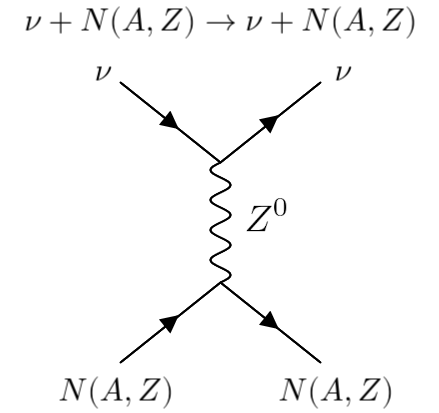
\includegraphics[width=\linewidth]{figures/feynman.png}
\label{fig:Feynmann_CEvNS}
\end{wrapfigure}
Coherent Elastic Neutrino-Nucleus Scattering (CE$\nu$NS) is a neutral current weak interaction within the SM originally proposed in 1979 \cite{PhysRevD.9.1389} and measured successfully in 2017 \cite{doi:10.1126/science.aao0990}, wherein low-energy neutrinos [$E_{\nu} \sim \, \text{MeV}$] collide with atomic nuclei as coherent bodies rather than their constituents, imparting on them a small recoil energy. These interactions are possible with neutrino energies up to $50\,MeV$ with medium-sized nuclei, since their main condition consists of the momentum transfer, $Q$, being negligible in comparison with the nuclear radius, $R$ ($QR \ll 1$) \cite{Scholberg_2020}. The effective Feynman diagram for these interactions is shown in Fig. \ref{fig:Feynmann_CEvNS}.

The calculation of its differential cross-section in the low-energy limit consists of setting an effective Lagrangian density given by:
\begin{equation}
    \mathcal{L_{\text{eff}}} = \frac{G}{\sqrt{2}}j^{(\nu)\mu} \mathcal{J}_{\mu},
\end{equation}
where $j^{(\nu)\mu}$ denotes a neutral neutrino current and $\mathcal{J}_{\mu}$ a hadronic current from which the nuclear mass distribution terms originate.
\section{Cross Section}
The low-energy differential cross-section in terms of the nuclear recoil, $E_R$, is given by \cite{Papoulias2015}:
\begin{equation}
    \frac{d\sigma}{dT}(E_\nu, E_R) = \frac{G_{F}^{2} M}{\pi}Q_{W}^{2}\left(1 - \frac{ME_R}{2E_\nu}\right),
\end{equation}
where $M$ is the target nuclear mass and $Q_W^2$ is the vector nuclear weak charge given in terms of the proton ($p$) and neutron ($n$) weak couplings:
\begin{equation}
    Q_{W}^{2} = [Zg^{p}_{V}F_p(q^2) + Ng^{n}_{V}F_n(q^2)]^2,
    \label{eq:QW}
\end{equation}
where $g^{p}_{V}$ and $g^{n}_{V}$ are given by (\ref{eq:gv}) in the specific cases for the proton and neutron respectively:
\begin{align}
    g^{p}_{V}   &= T^3_{p}-2\sin^2(\theta_W)Q_{p}   =\frac{1}{2} - 2\sin^2(\theta_W),&\label{eq:gVp}\\
    g^{n}_{V}   &= T^3_{n}-2\sin^2(\theta_W)Q_{n}  =-\frac{1}{2},& \label{eq:gVn}
\end{align}
and $F_{n,p}(Q^2)$ are the neutron and proton nuclear form factors, dependent on the momentum transfer $q^2 = 2MT$. In Eqs. (\ref{eq:QW}), (\ref{eq:gVp}), and (\ref{eq:gVn}), $Z$ is the atomic number, $N = A-Z$ is the neutron number, and $A$ is the mass (nucleon) number of the target nucleus. It is worth noting that, given the weak mixing angle $\sin^2(\theta_W) \approx 0.22290(30) \approx \frac{1}{4}$ \cite{RevModPhys.93.025010}, $Q_{W}^{2}$ (and by extension $\frac{d\sigma}{dT}$) is mostly $\propto N^2$.
\section{Neutrino Sources}
Part of the calculation of the expected number of CE$\nu$NS events is the energy-dependent flux of incoming (anti)neutrinos. This work focuses mainly on a model for electron-antineutrinos known as the Huber-Mueller model.
\subsection{Nuclear Reactors}
Ever since their discovery in 1959~\cite{doi:10.1126/science.124.3212.103}, reactor neutrino sources have been fundamental for neutrino physics. In recent times they have still been utilized in experiments such as the measurement of $\Delta m_{21}$ in KamLAND~\cite{Aliani_2004} and of the mixing angle $\theta_{13}$ in Daya Bay~\cite{dayabaycollaboration2007precision}. The main inspiration for the present work comes from two papers, one by L. J. Flores et al. \cite{Flores_2021} and another by E. Alfonso-Pita et al. \cite{Alfonso_Pita_2022}, wherein a 10 kg scintillating liquid Argon (LAr) bubble chamber detector is placed at a distance of $\sim$3 m from a reactor running at $\sim$1 MW$_{th}$ thermal power, based on a TRIGA Mark III nuclear reactor at the National Institute of Nuclear Research (ININ) facilities on the Mexico-Toluca highway near Mexico City.

Nuclear reactors commonly operate based on Uranium and Plutonium, whose fission produces a large quantity of neutron-rich remnant nuclei that subsequently undergo beta decay. The resulting antineutrino flux for $^{235}$U, $^{239}$Pu, and $^{241}$Pu has been calculated by the Institut Laue-Langevin (ILL) in the 1980s~\cite{VONFEILITZSCH1982162, SCHRECKENBACH1985325}. Coupled with an \textit{ab initio} method for the estimation of the $^{238}$U spectrum as seen in \cite{PhysRevD.70.053011}, the following model is obtained for the total electron antineutrino spectrum, known as the Huber-Mueller model~\cite{PhysRevC.83.054615}:
\begin{equation}
      \frac{d\Phi}{dE_\nu}(E_{\nu}) = \frac{P}{4 \pi d^2}\sum_{k}\frac{f_{k}}{\epsilon_{k}}\exp \left(\sum_{p=1}^{6}\alpha_{kp}E_{\nu}^{p-1}\right),
\end{equation}
where $P$ is the thermal power of the reactor, $d$ is the reactor-detector distance, $k \in \{ ^{235}\text{U}, ^{239}\text{Pu} , ^{241}\text{Pu}, ^{238}\text{U} \}$ is an index that runs through the contribution of the isotopes involved, $\epsilon_k$ is the energy per fission of each isotope as published in~\cite{Kopeikin2004}, $f_{k}$ is the fission fraction of each isotope, and $\alpha_{kp}$ are the experimentally fitted coefficients shown in Table \ref{tb:reactor_param}.
\setlength\tabcolsep{0pt}
\begin{table}
\begin{tabular*}{\linewidth}{@{\extracolsep{\fill}} cccccc }
\toprule
           & $^{235}$U             & $^{238}$U             & $^{239}$Pu            & $^{241}$Pu            \\ \midrule
$\alpha_1$ & 3.217                 & 4.833$\cdot 10^{-1}$  & 6.413                 & 3.251                 \\
$\alpha_2$ & -3.111                & 1.927$\cdot 10^{-1}$  & -7.432                & -3.204                \\
$\alpha_3$ & 1.395                 & -1.283$\cdot 10^{-1}$ & 3.535                 & 1.428                 \\
$\alpha_4$ & -3.690$\cdot 10^{-1}$ & -6.762$\cdot 10^{-3}$ & -8.820$\cdot 10^{-1}$ & -3.675$\cdot 10^{-1}$ \\
$\alpha_5$ & 4.445$\cdot 10^{-2}$  & 2.233$\cdot 10^{-3}$  & 1.025$\cdot 10^{-1}$  & 4.254$\cdot 10^{-2}$  \\
$\alpha_6$ & -2.053$\cdot 10^{-3}$ & -1.536$\cdot 10^{-4}$ & -4.550$\cdot 10^{-3}$ & -1.869$\cdot 10^{-3}$ \\ \bottomrule
\end{tabular*}

\caption{Experimentally fitted coefficients $\alpha_{kp}$ as published in \cite{PhysRevC.83.054615}.}
\label{tb:reactor_param}
\end{table}
\noindent In Fig. \ref{fig:reator_sperate} the individual isotope contributions are plotted against each other in arbitrary units, and Fig. \ref{fig:reator_total} shows the total flux given the fission fractions: 55$\%$ of $^{235}$U, 32$\%$ of $^{239}$Pu, 6$\%$ of $^{241}$Pu, and 7$\%$ of $^{238}$U, in accordance with \cite{Wong_2007}.

\begin{figure}
    \centering
    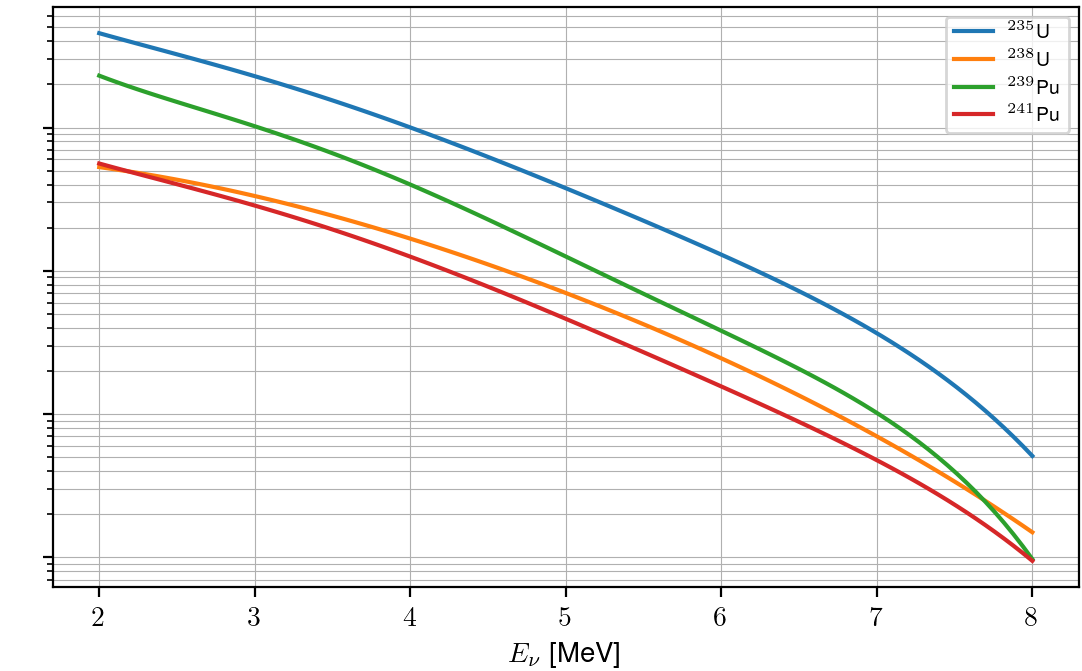
\includegraphics[width=0.8\textwidth]{figures/reactor_separate_crop.png}
    \caption{Isotope contributions to total antineutrino flux spectrum.}
    \label{fig:reator_sperate}
\end{figure}

\begin{figure}
    \centering
    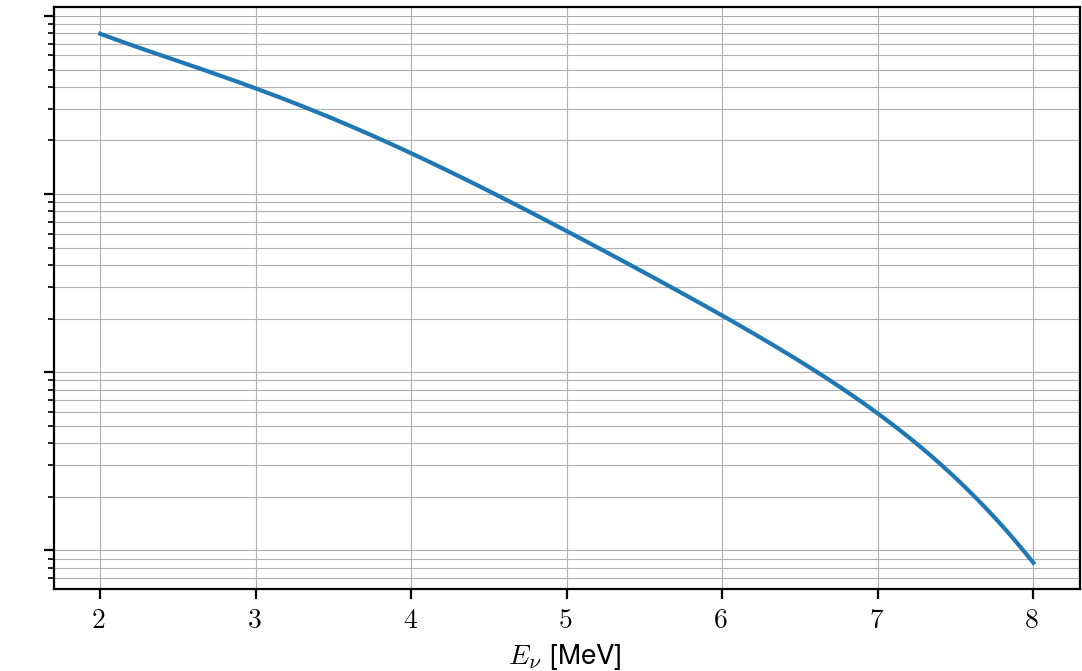
\includegraphics[width=0.8\textwidth]{figures/reactor_total_crop.png}
    \caption{Total antineutrino flux spectrum.}
    \label{fig:reator_total}
\end{figure}

\section{Expected Number of Events}
Ignoring reactor resolution and efficiency, the expected number of events of a detector of mass $M$ over an exposure time $t$ is given by
\begin{equation}
    N =  t\frac{M_{\text{Detector}}}{M}\int_{E_{R\text{ th}}}^{E_{R\text{ max}}}dE_R\int_{E_{\nu, \text{min}}(E_R)}^{E_{\nu,\text{max}}}dE_{\nu} \frac{d\Phi}{dE_\nu} (E_{\nu})\left( \frac{d\sigma}{dE_R}\right),
    \label{eq:N_events}
\end{equation}
where $E_{R\text{ th}}$ a threshold nuclear recoil energy, $E_{R\text{ max}}$ a kinematically determined maximum recoil energy, $E_{\nu,\text{max}}\sim9.5$ MeV the maximum incident neutrino energy given by the neutrino spectrum~\cite{SCHRECKENBACH1985325} and $E_{\nu, \text{min}}(E_R)\approx \sqrt{ME_R/2}$ the minimum incident neutrino energy required to produce a given $E_R$ recoil energy
\begin{equation}
    E_{\nu,\text{min}}(E_{R}) = \frac{E_{R}}{2}\left(1+\sqrt{1+\frac{2M}{E_{R}}}\right).
\end{equation}

    \chapter{Sensitivities for SBC-ININ-LAr Experiment}\label{cap:analisis}
\label{chap:sensitivity_sin2thetaW_NCR}

\section{Introduction}
This chapter presents the projected statistical sensitivity of a coherent elastic neutrino-nucleus scattering (CE$\nu$NS) experiment based on LAr target exposed to reactor antineutrinos, to two Standard Model parameters: the weak mixing angle $\sin^2\theta_W$ and the electron neutrino charge radius (NCR) $\langle r_{\nu_e}^2\rangle$. The results below correspond to different detector masses (10, 20, 100 and 200 kg), exposure times (100 and 200 days), and to the two limiting treatments of the QF discussed in the methodology chapter: an idealized QF $=1$ case and the realistic case computed from the Lindhard model for argon. The chapter reproduces the projected event rates, the $1\sigma$ confidence intervals extracted from the $\Delta\chi^2$ statistic, and the corresponding $\Delta\chi^2$ curves for each configuration.

\section{Calculation Parameters}
The results quoted throughout this chapter use the fixed inputs:
\begin{itemize}
\item $P = 1$ MW 
\item $d = 3$ m 
\item $t = 100$ or $200$ days 
\item $M_{\text{Detector}} = 20$, $100$ or $200$ kg 
\item $N_{\text{targets}} = 3\times10^{26}$ 
\item $1.5\times10^{27}$ or $3\times10^{27}$ 
\item $M = 39.95$ u $= 37.21$ GeV for the $^{40}$Ar nucleus 
\item $M_W = 80.379$ GeV, $G_F = 1.16\times10^{-11}\ \text{MeV}^{-2}$ 
\item $g_n^V = -\tfrac{1}{2}$ 
\end{itemize}
together with the Standard Model reference values $\left(\sin^2\theta_W\right)_{\text{SM}} = 0.22337$ and $\langle r_{\nu_e}^2\rangle_{\text{SM}} = -0.826\times10^{-32}\ \text{cm}^2$. The differential event rate follows the usual CE$\nu$NS convolution of the Huber-Mueller reactor flux with the CE$\nu$NS cross section, integrated over the recoil-energy window set by the ionization threshold $E_{I}^{\text{threshold}} \sim 100\ \text{eV}_{\text{ee}}$, which through the Lindhard quenching relation corresponds to $E_{R}^{\text{threshold}} \sim 400\ \text{eV}_{\text{nr}}$.

\section{Projected Event Rates}
Table~\ref{tab:event_rates} lists the expected number of events per day for each detector mass, separately for the two parametrizations of $g_p^V$ (pure $\sin^2\theta_W$ dependence, and the combined $\sin^2\theta_W$-NCR dependence), and for the two QF treatments.

\begin{table}[H]
\centering
\caption{Projected CE$\nu$NS event rates (events/day) as a function of detector mass, for $QF=1$ and for the Lindhard quenching model.}
\label{tab:event_rates}
\begin{tabular}{lcccc}
\hline
$g_p^V$ ($QF=1$) & 10 kg & 20 kg & 100 kg & 200 kg \\
\hline
$\propto \sin^2\theta_W$ & $\sim 10.1$ & $\sim 20.2$ & $\sim 101$ & $\sim 202$ \\
$\propto \sin^2\theta_W\left(1+\tfrac{1}{3}M_W^2\langle r_{\nu_e}^2\rangle\right)$ & $\sim 10.5$ & $\sim 21.1$ & $\sim 105$ & $\sim 211$ \\
\hline
\hline
$g_p^V$ (Lindhard QF) & 10 kg & 20 kg & 100 kg & 200 kg \\
\hline
$\propto \sin^2\theta_W$ & $\sim 2.2$ & $\sim 4.5$ & $\sim 22$ & $\sim 44$ \\
$\propto \sin^2\theta_W\left(1+\tfrac{1}{3}M_W^2\langle r_{\nu_e}^2\rangle\right)$ & $\sim 2.3$ & $\sim 4.7$ & $\sim 23$ & $\sim 46$ \\
\hline
\end{tabular}
\end{table}

The reduction of roughly a factor of $4$-$5$ in the expected rate between the $QF=1$ and Lindhard cases reflects the fraction of recoil events lost below the ionization threshold once the realistic quenching relation is applied, and it propagates directly into the widths of the confidence intervals discussed below.

\section{Results}
All intervals below are quoted at $68.27\%$ confidence level ($1\sigma$), obtained from the $\Delta\chi^2$ statistic defined in the methodology chapter, without including systematic correlations between $\sin^2\theta_W$ and $\langle r_{\nu_e}^2\rangle$.

\subsection{Without QF Influence}

\subsubsection{Sensitivity to \texorpdfstring{$\sin^2\theta_W$}{sin2thetaW}}
For an experiment with 100-day exposure and $QF=1$, the values at $1\sigma$ confidence level are given by:
\begin{itemize}
\item $\sin^2\theta_W = 0.223\pm0.007$, 10 kg detector.
\item $\sin^2\theta_W = 0.223\pm0.005$, 20 kg detector.
\item $\sin^2\theta_W = 0.223\pm0.003$, 100 kg detector.
\item $\sin^2\theta_W = 0.223\pm0.001$, 200 kg detector.
\end{itemize}

% \begin{figure}[H]
% \centering
% 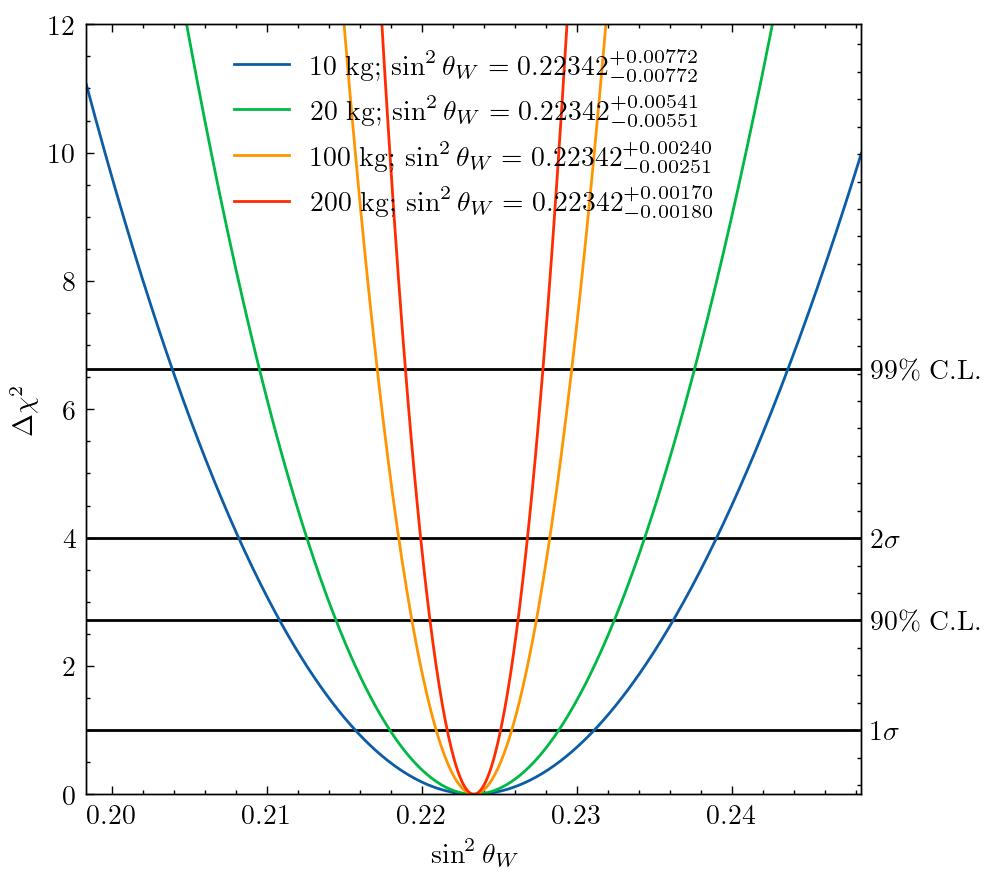
\includegraphics[width=0.5\textwidth]{figures/Figure_sin_100_NO_QF.png}
% \caption{$\Delta\chi^2$ curves for the parameter $\sin^2\theta_W$, experimental arrangement with 100-day exposure.}
% \label{fig:chi2_sin2thetaW_100d}
% \end{figure}

For an experiment with 200-day exposure and $QF=1$, the values at $1\sigma$ confidence level are given by:
\begin{itemize}
\item $\sin^2\theta_W = 0.223\pm0.005$, 10 kg detector.
\item $\sin^2\theta_W = 0.223\pm0.003$, 20 kg detector.
\item $\sin^2\theta_W = 0.223\pm0.002$, 100 kg detector.
\item $\sin^2\theta_W = 0.223\pm0.001$, 200 kg detector.
\end{itemize}

% \begin{figure}[H]
% \centering
% 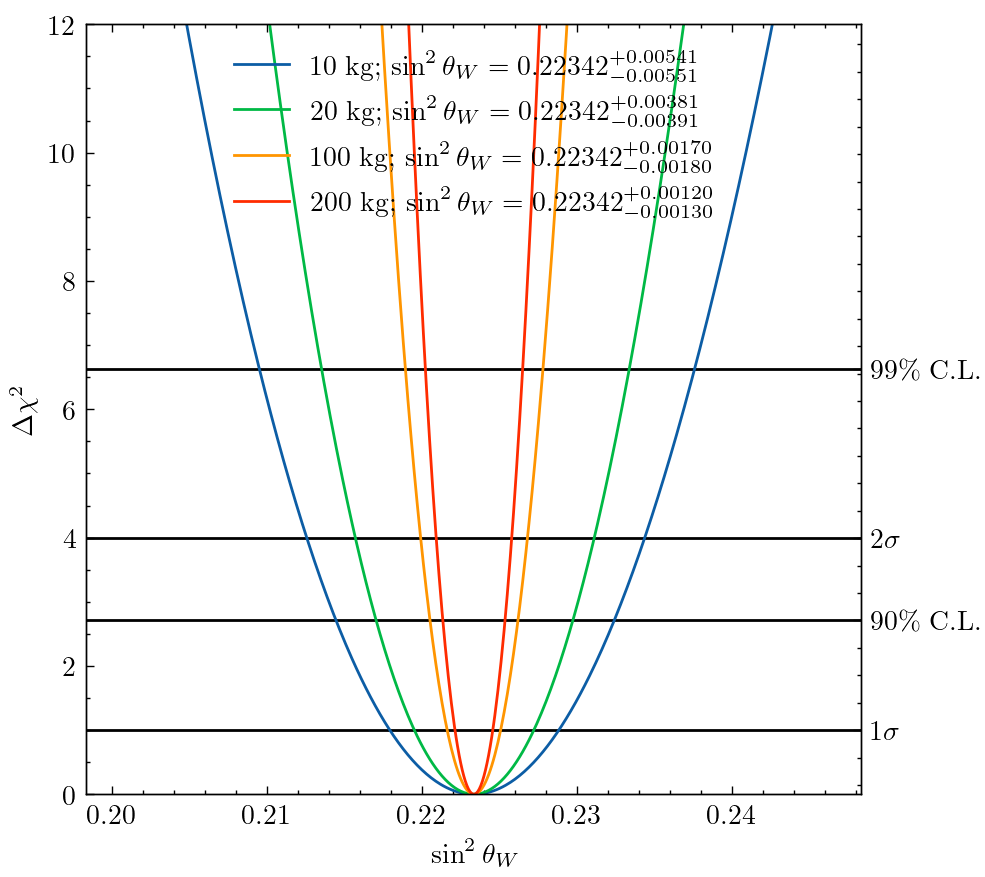
\includegraphics[width=0.5\textwidth]{figures/Figure_sin_200_NO_QF.png}
% \caption{$\Delta\chi^2$ curves for the parameter $\sin^2\theta_W$, experimental arrangement with 200-day exposure.}
% \label{fig:chi2_sin2thetaW_200d}
% \end{figure}

\begin{figure}[H]
\centering
\subfigure[100-day exposure.]{
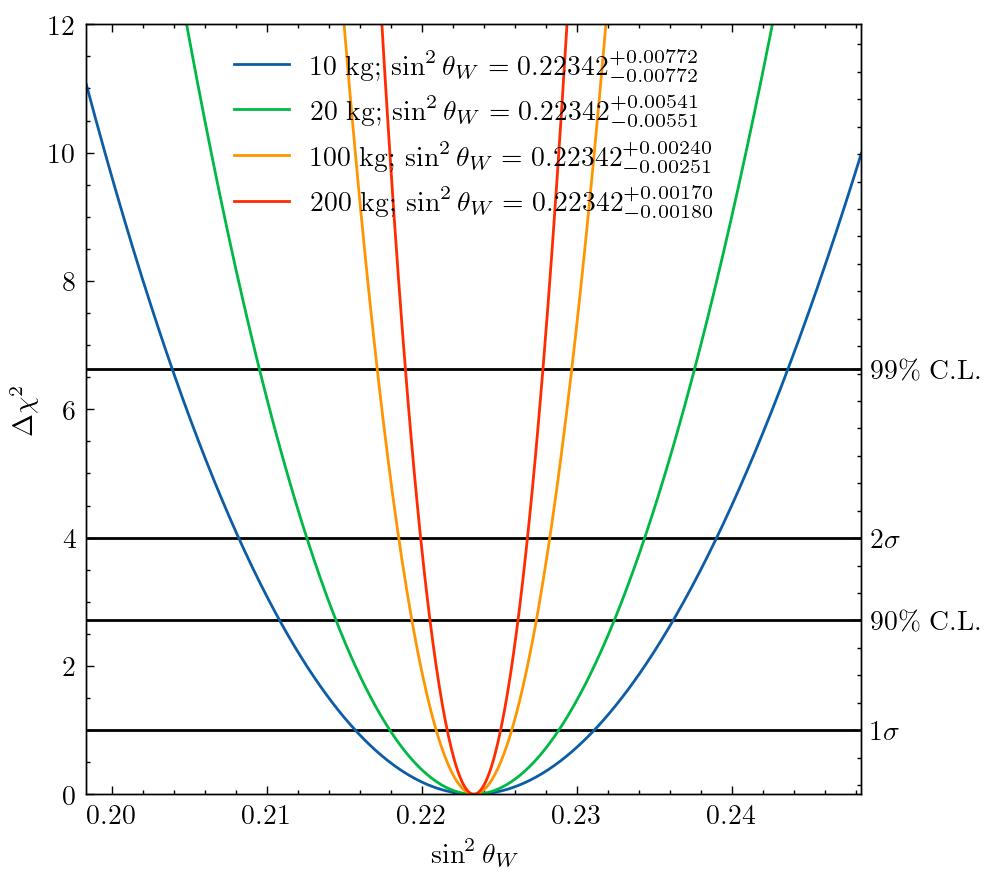
\includegraphics[width=0.48\textwidth]{figures/Figure_sin_100_NO_QF.png}
\label{fig:chi2_sin2thetaW_100d}}
\subfigure[200-day exposure.]{
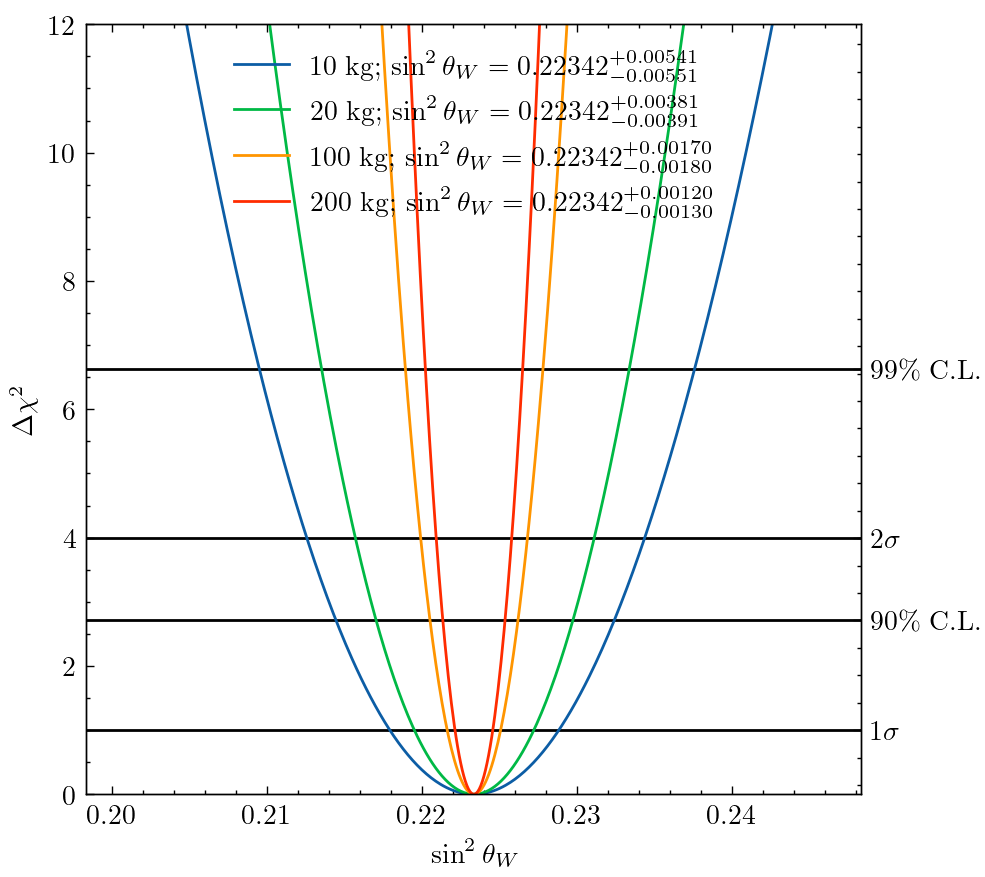
\includegraphics[width=0.48\textwidth]{figures/Figure_sin_200_NO_QF.png}
\label{fig:chi2_sin2thetaW_200d}}
\caption{$\Delta\chi^2$ curves for the parameter $\sin^2\theta_W$, without QF influence.}
\label{fig:chi2_sin2thetaW_noQF}
\end{figure}


\subsubsection{Sensitivity to \texorpdfstring{$\langle r_{\nu_e}^2\rangle$}{NCR}}
For an experiment with 100-day exposure and $QF=1$, the values at $1\sigma$ confidence level are given by:
\begin{itemize}
\item $\langle r_{\nu_e}^2\rangle = -8\pm6\times10^{-33}\ \text{cm}^2$, 10 kg detector.
\item $\langle r_{\nu_e}^2\rangle = -8\pm4\times10^{-33}\ \text{cm}^2$, 20 kg detector.
\item $\langle r_{\nu_e}^2\rangle = -8\pm2\times10^{-33}\ \text{cm}^2$, 100 kg detector.
\item $\langle r_{\nu_e}^2\rangle = -8\pm1\times10^{-33}\ \text{cm}^2$, 200 kg detector.
\end{itemize}

% \begin{figure}[H]
% \centering
% 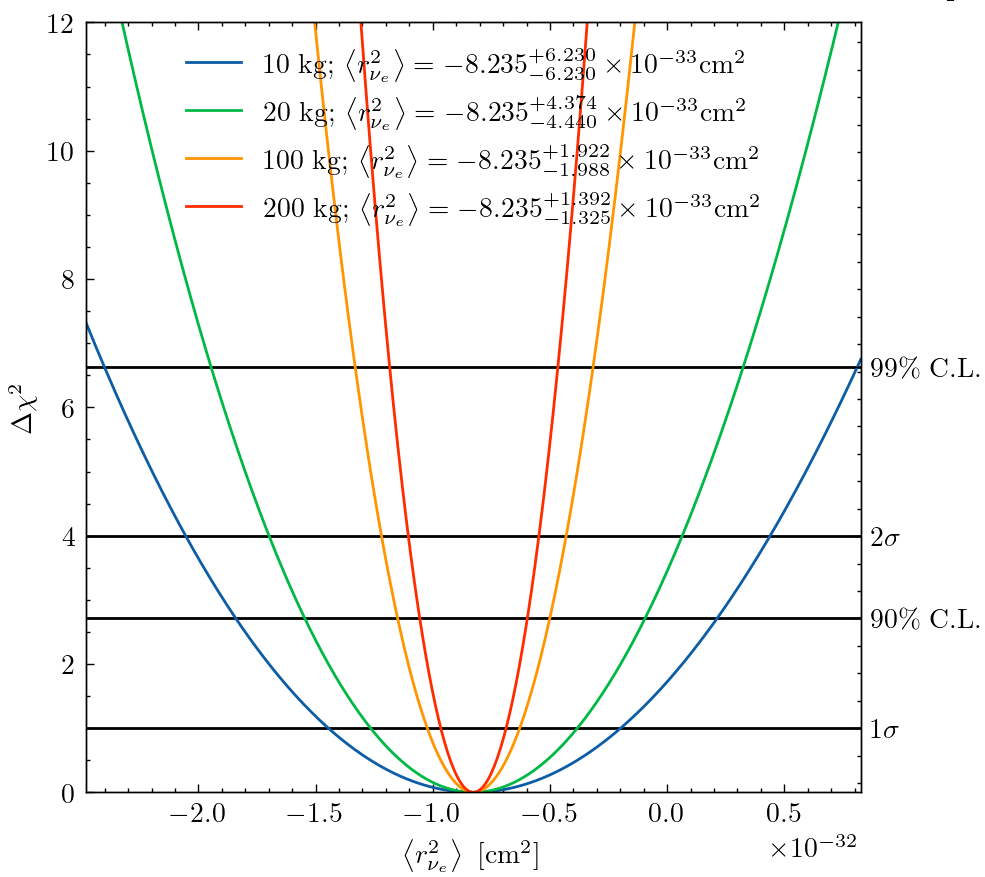
\includegraphics[width=0.5\textwidth]{figures/Figure_phi_100_NO_QF.png}
% \caption{$\Delta\chi^2$ curves for the parameter $\langle r_{\nu_e}^2\rangle$, experimental arrangement with 100-day exposure.}
% \label{fig:chi2_NCR_100d}
% \end{figure}

or an experiment with 200-day exposure and $QF=1$, the values at $1\sigma$ confidence level are given by:
\begin{itemize}
\item $\langle r_{\nu_e}^2\rangle = -8\pm4\times10^{-33}\ \text{cm}^2$, 10 kg detector.
\item $\langle r_{\nu_e}^2\rangle = -8\pm3\times10^{-33}\ \text{cm}^2$, 20 kg detector.
\item $\langle r_{\nu_e}^2\rangle = -8\pm1\times10^{-33}\ \text{cm}^2$, 100 kg detector.
\item $\langle r_{\nu_e}^2\rangle = -8.2\pm0.9\times10^{-33}\ \text{cm}^2$, 200 kg detector.
\end{itemize}

\begin{figure}[H]
\centering
\subfigure[100-day exposure.]{
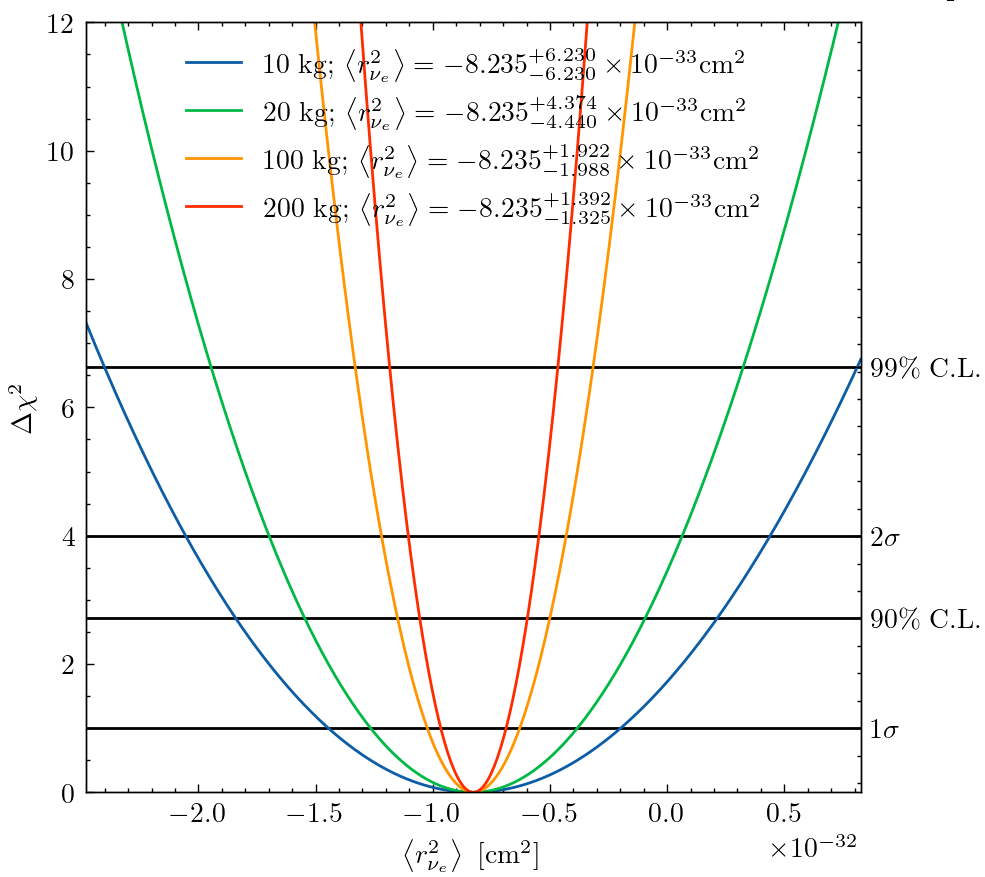
\includegraphics[width=0.48\textwidth]{figures/Figure_phi_100_NO_QF.png}
\label{fig:chi2_sin2thetaW_100d}}
\subfigure[200-day exposure.]{
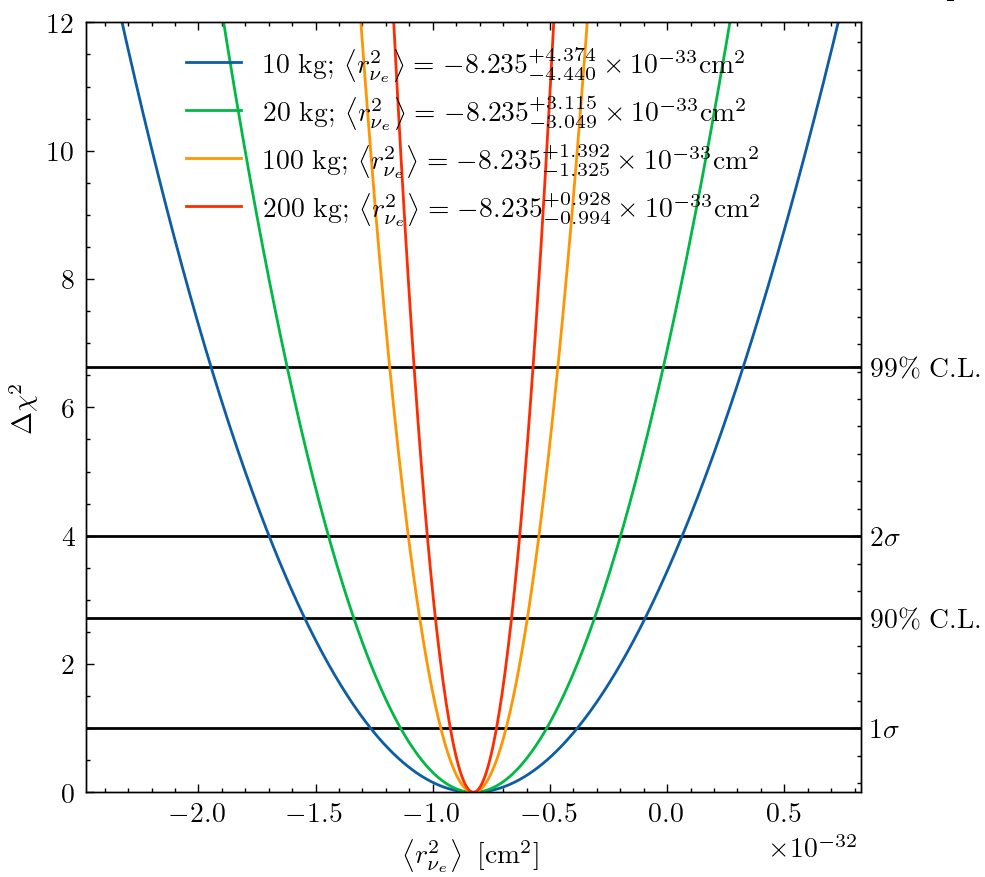
\includegraphics[width=0.48\textwidth]{figures/Figure_phi_200_NO_QF.png}
\label{fig:chi2_sin2thetaW_200d}}
\caption{$\Delta\chi^2$ curves for the parameter $\langle r^2_{\nu_e} \rangle$, without QF influence.}
\label{fig:chi2_sin2thetaW_noQF}
\end{figure}

\subsection{With QF Influence}

\subsubsection{Sensitivity to \texorpdfstring{$\sin^2\theta_W$}{sin2thetaW}}
Including the Lindhard quenching factor, the 100-day exposure yields 

$\sin^2\theta_W = 0.22\pm0.02$, 10 kg detector. 
$\sin^2\theta_W = 0.22\pm0.01$, 20 kg detector.
$\sin^2\theta_W = 0.223\pm0.005$, 100 kg detector. 
$\sin^2\theta_W = 0.223\pm0.003$, 200 kg detector.

% \begin{figure}[H]
% \centering
% 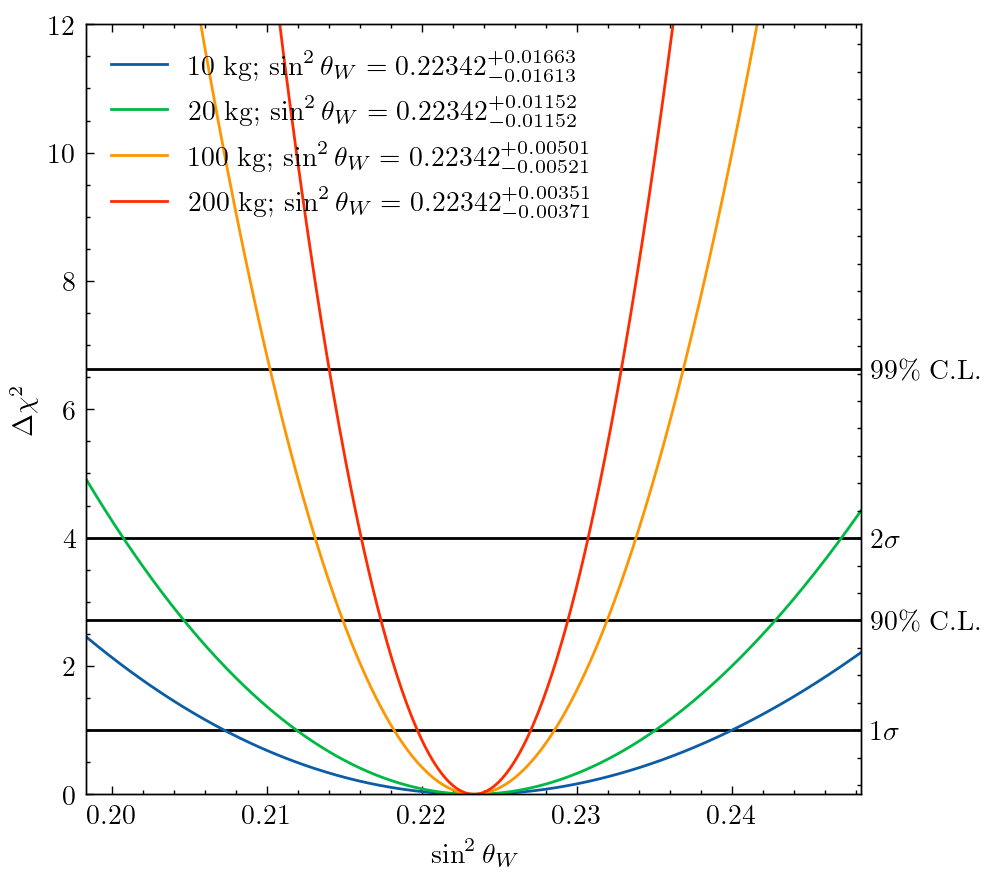
\includegraphics[width=0.5\textwidth]{figures/Figure_sin_100.png}
% \caption{$\Delta\chi^2$ curves for the parameter $\sin^2\theta_W$, experimental arrangement with 100-day exposure, including quenching factor.}
% \label{fig:chi2_sin2thetaW_100d_QF}
% \end{figure}

For an experiment with 200-day exposure, including the Lindhard quenching factor, the values at $1\sigma$ confidence level are given by:
\begin{itemize}
\item $\sin^2\theta_W = 0.22\pm0.01$, 10 kg detector.
\item $\sin^2\theta_W = 0.223\pm0.008$, 20 kg detector.
\item $\sin^2\theta_W = 0.223\pm0.003$, 100 kg detector.
\item $\sin^2\theta_W = 0.223\pm0.002$, 200 kg detector.
\end{itemize}

\begin{figure}[H]
\centering
\subfigure[100-day exposure.]{
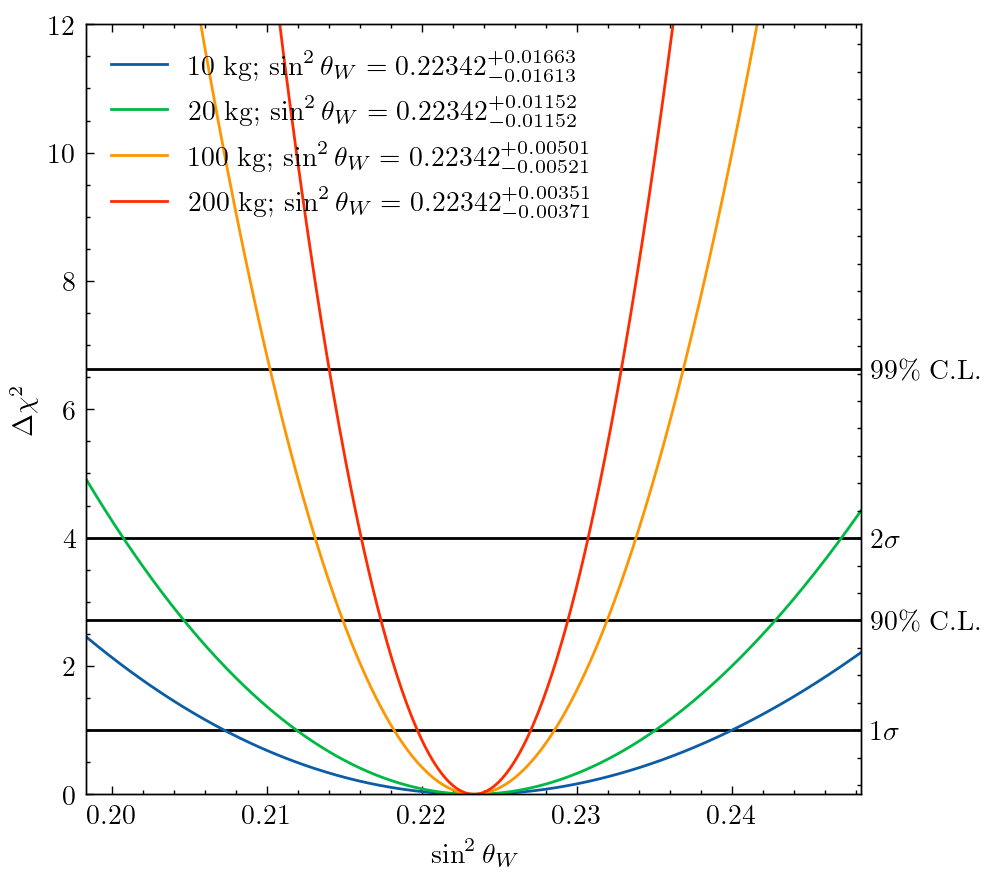
\includegraphics[width=0.48\textwidth]{figures/Figure_sin_100.png}
\label{fig:chi2_sin2thetaW_100d}}
\subfigure[200-day exposure.]{
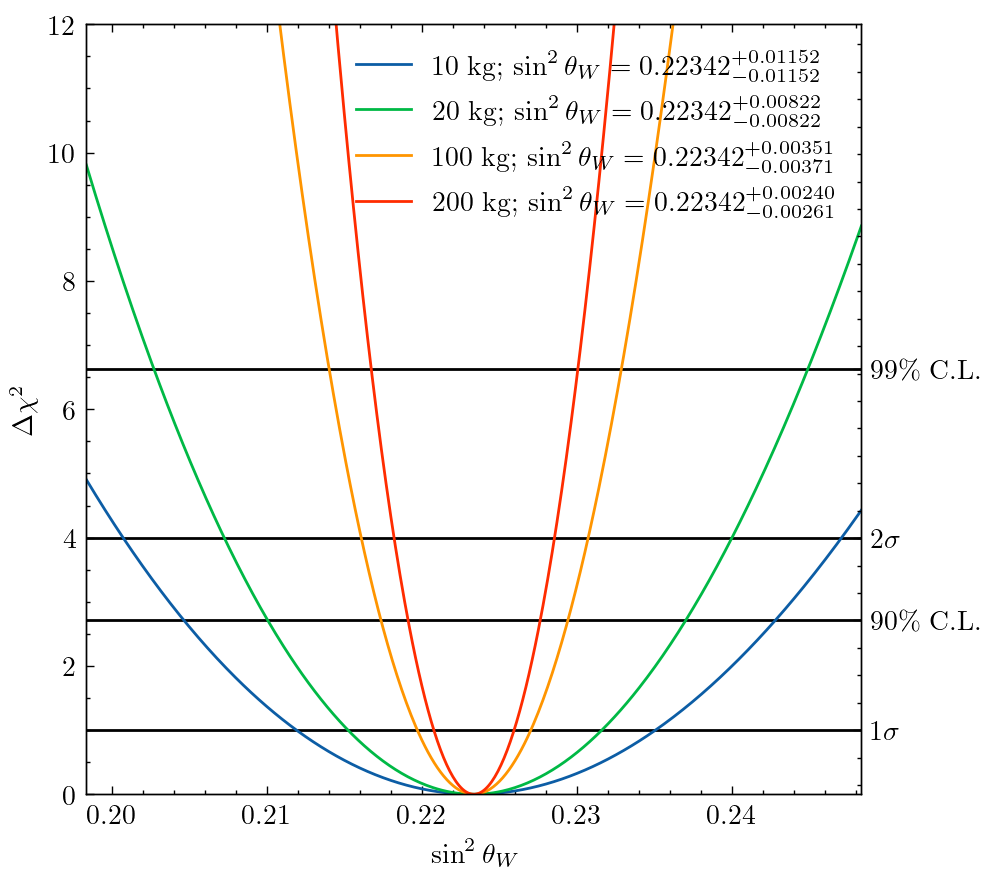
\includegraphics[width=0.48\textwidth]{figures/Figure_sin_200.png}
\label{fig:chi2_sin2thetaW_200d}}
\caption{$\Delta\chi^2$ curves for the parameter $\sin^2 \theta_W$, with Lindhard QF influence.}
\label{fig:chi2_sin2thetaW_noQF}
\end{figure}

% \begin{figure}[H]
% \centering
% 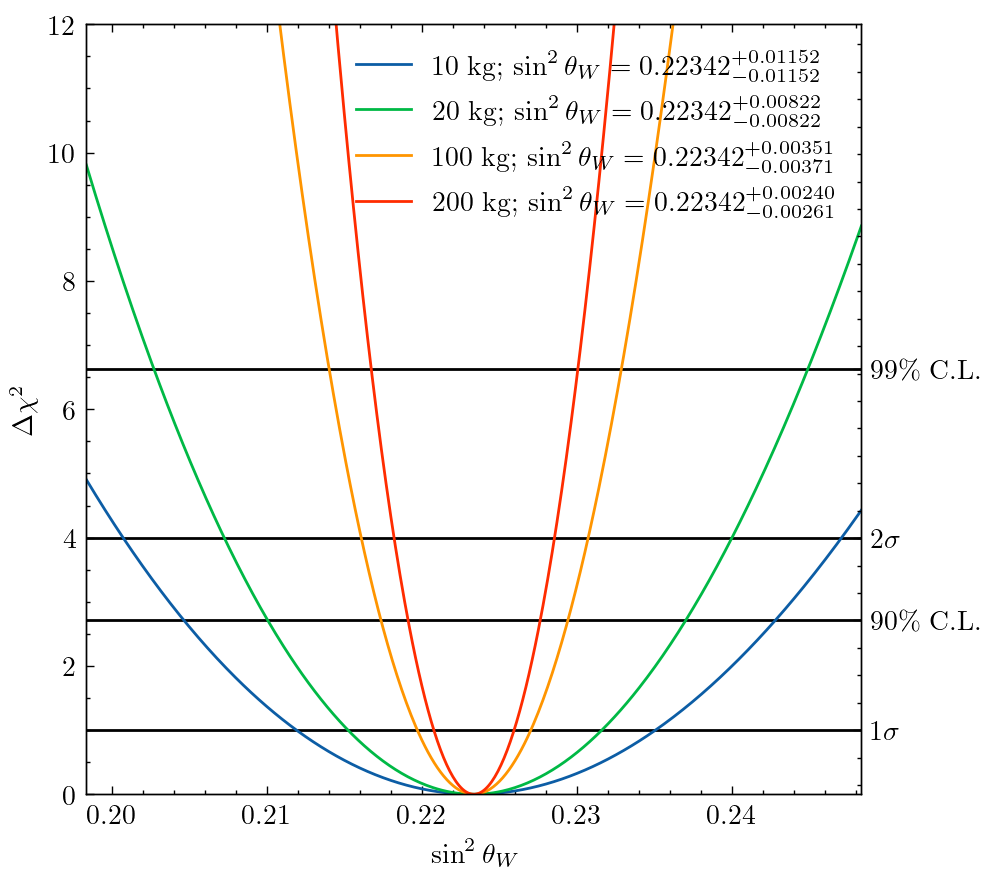
\includegraphics[width=0.5\textwidth]{figures/Figure_sin_200.png}
% \caption{$\Delta\chi^2$ curves for the parameter $\sin^2\theta_W$, experimental arrangement with 200-day exposure, including quenching factor.}
% \label{fig:chi2_sin2thetaW_200d_QF}
% \end{figure}



\subsubsection{Sensitivity to \texorpdfstring{$\langle r_{\nu_e}^2\rangle$}{NCR}}

For an experiment with 100-day exposure, including the Lindhard quenching factor, the values at $1\sigma$ confidence level are given by:
\begin{itemize}
\item $\langle r_{\nu_e}^2\rangle = -8\pm13\times10^{-33}\ \text{cm}^2$, 10 kg detector.
\item $\langle r_{\nu_e}^2\rangle = -8\pm9\times10^{-33}\ \text{cm}^2$, 20 kg detector.
\item $\langle r_{\nu_e}^2\rangle = -8\pm4\times10^{-33}\ \text{cm}^2$, 100 kg detector.
\item $\langle r_{\nu_e}^2\rangle = -8\pm3\times10^{-33}\ \text{cm}^2$, 200 kg detector.
\end{itemize}

% \begin{figure}[H]
% \centering
% 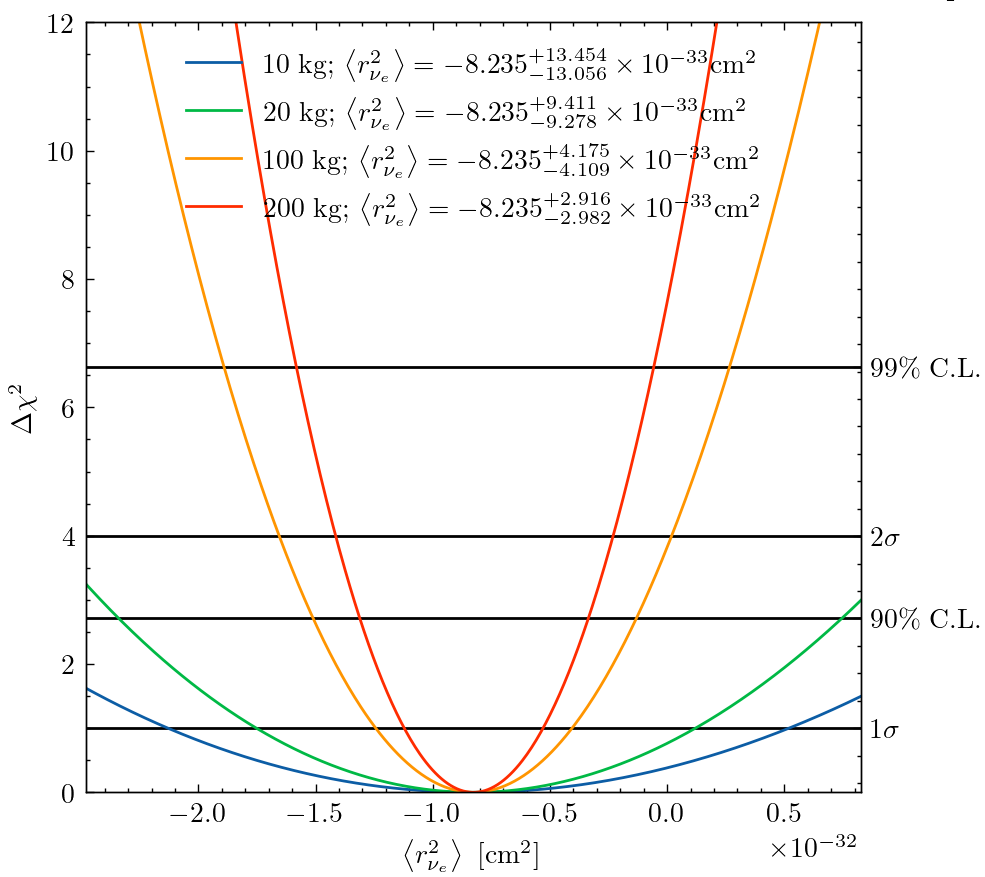
\includegraphics[width=0.5\textwidth]{figures/Figure_phi_100.png}
% \caption{$\Delta\chi^2$ curves for the parameter $\langle r_{\nu_e}^2\rangle$, experimental arrangement with 100-day exposure, including quenching factor.}
% \label{fig:chi2_NCR_100d_QF}
% \end{figure}

For an experiment with 200-day exposure, including the Lindhard quenching factor, the values at $1\sigma$ confidence level are given by:
\begin{itemize}
\item $\langle r_{\nu_e}^2\rangle = -8\pm9\times10^{-33}\ \text{cm}^2$, 10 kg detector.
\item $\langle r_{\nu_e}^2\rangle = -8\pm6\times10^{-33}\ \text{cm}^2$, 20 kg detector.
\item $\langle r_{\nu_e}^2\rangle = -8\pm3\times10^{-33}\ \text{cm}^2$, 100 kg detector.
\item $\langle r_{\nu_e}^2\rangle = -8\pm2\times10^{-33}\ \text{cm}^2$, 200 kg detector.
\end{itemize}


% \begin{figure}[H]
% \centering
% 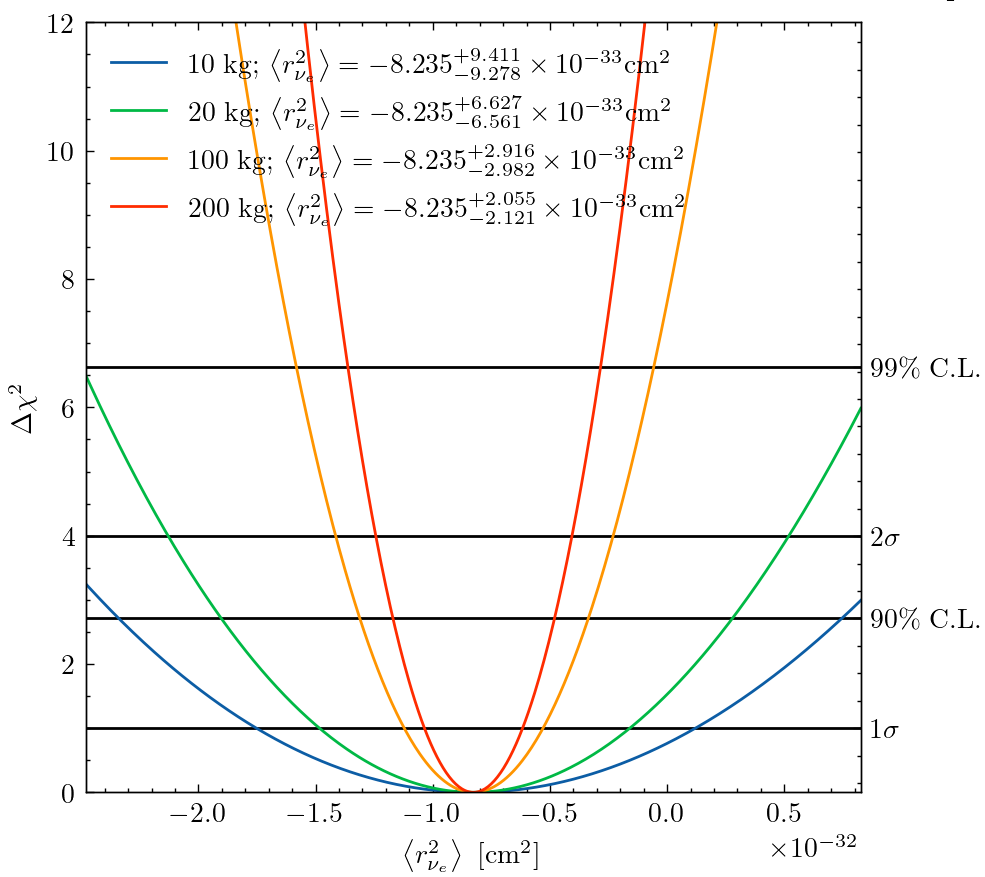
\includegraphics[width=0.5\textwidth]{figures/Figure_phi_200.png}
% \caption{$\Delta\chi^2$ curves for the parameter $\langle r_{\nu_e}^2\rangle$, experimental arrangement with 200-day exposure, including quenching factor.}
% \label{fig:chi2_NCR_200d_QF}
% \end{figure}


\begin{figure}[H]
\centering
\subfigure[100-day exposure.]{
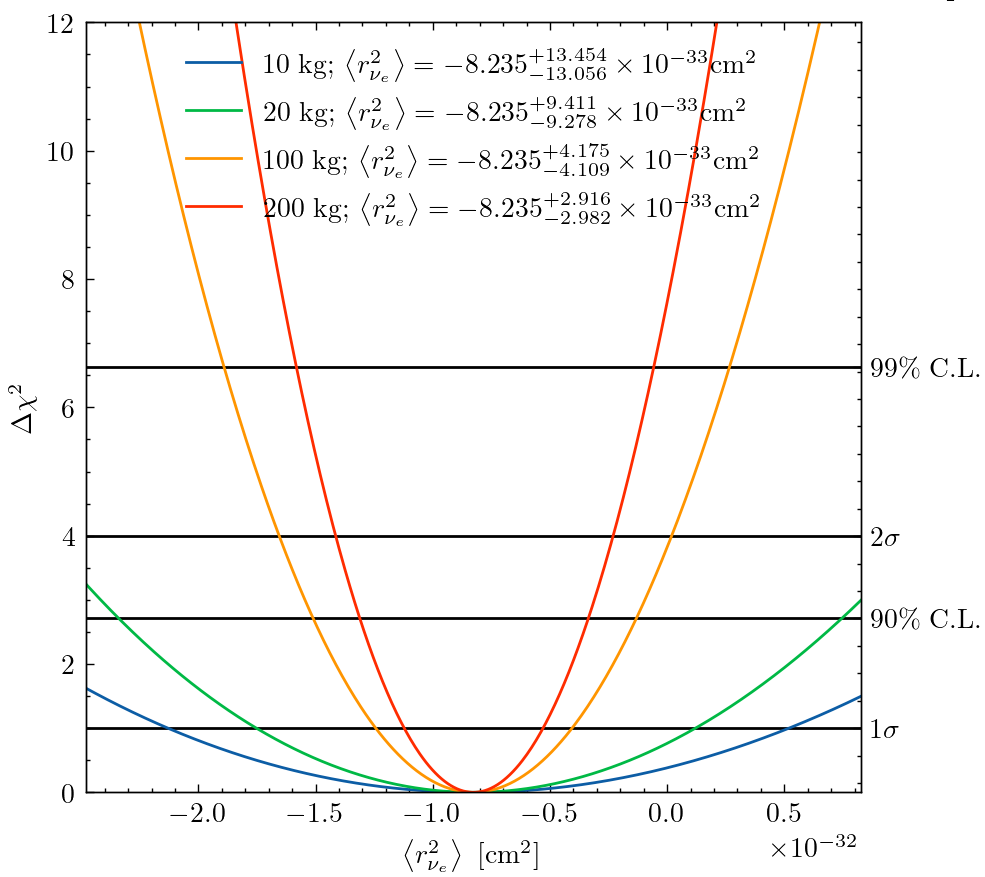
\includegraphics[width=0.48\textwidth]{figures/Figure_phi_100.png}
\label{fig:chi2_sin2thetaW_100d}}
\subfigure[200-day exposure.]{
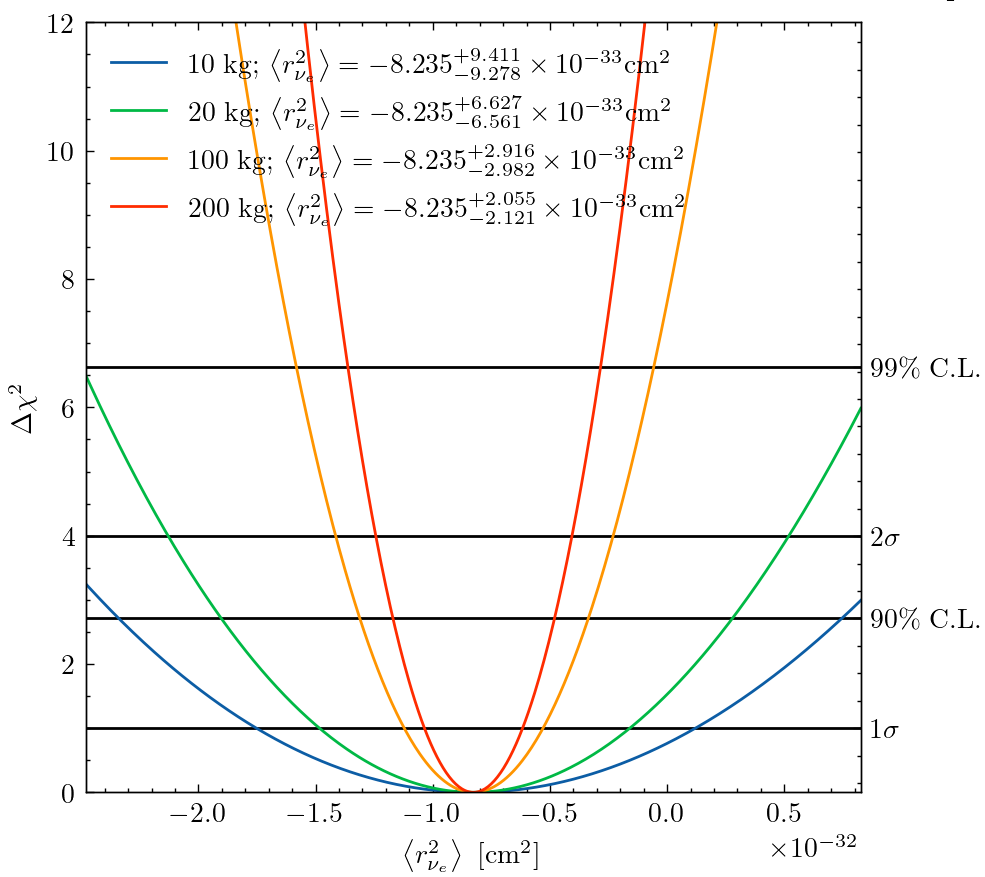
\includegraphics[width=0.48\textwidth]{figures/Figure_phi_200.png}
\label{fig:chi2_sin2thetaW_200d}}
\caption{$\Delta\chi^2$ curves for the parameter $\langle r^2_{\nu_e} \rangle$, with Lindhard QF influence.}
\label{fig:chi2_sin2thetaW_noQF}
\end{figure}

    \newpage{\ }
    \thispagestyle{empty}
    \chapter{Summary and conclusions}\label{chap:summary_conclusions}
Coherent Elastic Neutrino-Nucleus Scattering (CE$\nu$NS) provides a uniquely clean laboratory for probing the electroweak sector of the Standard Model (SM) at low momentum transfer, since its cross section factorizes into a coherently enhanced nuclear form factor and a weak charge that carries the full dependence on the underlying couplings. In this work we exploited that sensitivity to study two related, and often degenerate, SM quantities: the weak mixing angle $\sin^2\theta_W$ and the electron neutrino charge radius (NCR) $\langle r_{\nu_e}^2\rangle$, using a liquid argon (LAr) detector exposed to the antineutrino flux of a research reactor. We began by tracing the historical and formal path that leads from Fermi's effective four-fermion interaction, through the V-A structure, the $SU(2)_L$ gauge construction, and the neutral-current and Higgs discoveries, to the modern electroweak Lagrangian, in order to motivate the neutrino electromagnetic form factors, and in particular the charge radius, as a natural and gauge-invariant extension of that framework rather than an ad hoc addition. Within that formalism we detailed the Dirac and Weyl cases for the NCR, and we clarified the numerical relation between the two conventions most commonly found in the literature, those of Bernab\'eu et al. and of Cadeddu et al., which differ by a factor of $-2$ and have historically been a source of confusion when comparing bounds across experiments.

We then derived, and made explicit, how a nonzero NCR modifies the effective proton vector coupling $g_p^V$ that enters the CE$\nu$NS cross section, inducing a calculable shift that is degenerate, at leading order, with a shift in $\sin^2\theta_W$ itself. This degeneracy is the central technical difficulty of the analysis, and it motivated the two complementary strategies pursued in this thesis: constraining $\sin^2\theta_W$ under the assumption of a SM NCR, and constraining $\langle r_{\nu_e}^2\rangle$ under the assumption of the SM weak mixing angle, for a family of realistic experimental configurations. The event rate was computed from the convolution of the Huber-Mueller reactor antineutrino flux model with the CE$\nu$NS differential cross section on $^{40}$Ar, for a detector placed 3 m from the core of the TRIGA Mark III reactor at ININ, near Mexico City, a compact and accessible neutrino source well suited to a staged, moderate-scale detector program.

A significant part of the analysis was devoted to the treatment of the detector response through the Lindhard quenching factor for argon, including the correct Jacobian treatment required to invert the relation between nuclear recoil energy and observed ionization energy. This step is not a minor technical detail: our results show that including the realistic quenching relation, rather than assuming an idealized unit response, degrades the projected precision on both $\sin^2\theta_W$ and $\langle r_{\nu_e}^2\rangle$ by a factor of two to three, since the low-energy recoils where the parameter dependence is most pronounced are precisely those most affected by quenching near threshold. We computed the projected $1\sigma$ sensitivities from a $\Delta\chi^2$ statistic, without correlations, for detector masses ranging from 10 to 200 kg and exposure times of 100 and 200 days. As expected from Poisson statistics, the sensitivity improves close to $1/\sqrt{N}$ with increasing exposure and close to an order of magnitude across the full mass range considered, with a 200 kg detector run for 200 days projected to reach a precision of order $1$-$2\%$ on $\sin^2\theta_W$ and of order $2\times10^{-33}\ \text{cm}^2$ on $\langle r_{\nu_e}^2\rangle$ even under the realistic quenching scenario. These figures place a reactor-based LAr array in a competitive, if not leading, position relative to existing low-energy determinations of the weak mixing angle, and they establish a concrete, testable target for the electron neutrino charge radius using a source and detector technology already available at a national laboratory scale.

Taken together, these results confirm that a modest, single-technology detector array is sufficient to place meaningful, simultaneous constraints on $\sin^2\theta_W$ and $\langle r_{\nu_e}^2\rangle$ from reactor CE$\nu$NS, provided that the quenching response is modeled with care and that exposure and target mass are pushed toward the upper end of what is technically feasible. The analysis presented here is, by design, a first approximation: it does not yet include full covariance between $\sin^2\theta_W$ and the NCR, nor does it explore additional flavor structure or physics beyond the Standard Model. Breaking the residual degeneracy between these two parameters, and extending the sensitivity study to the muon and tau neutrino charge radii and to non-standard neutrino interactions, is the natural continuation of this program, and it is precisely the direction outlined in the doctoral protocol that follows this thesis, which proposes a systematic, multi-flavor and multi-experiment study of the neutrino charge radius across SBC, CONUS+, IsoDAR, and DUNE. Each of these experiments probes a different combination of flux, target, and baseline, and a combined treatment across them, informed by the methodology developed here for the reactor-LAr case, offers a realistic path toward disentangling the weak mixing angle from the neutrino electromagnetic structure and toward constraining genuinely new physics in the neutrino sector.
    \newpage{\ }
    \thispagestyle{empty}


    % Bibliografía
    
    \printbibliography[heading=bibintoc]
        

% Fin del documento
\end{document}
